\documentclass[11pt, a4paper, twoside]{book}

\setlength{\topmargin}{2pt} \setlength{\headheight}{15pt}
\setlength{\headsep}{25pt} \setlength{\textheight}{640pt}
\setlength{\footskip}{25pt}
\setlength{\hoffset}{0pt}
\setlength{\oddsidemargin}{0pt} \setlength{\oddsidemargin}{3pt}
\setlength{\evensidemargin}{0pt} \setlength{\evensidemargin}{30pt}
\setlength{\textwidth}{430pt}
\setlength{\marginparsep}{0pt} \setlength{\marginparwidth}{0pt}
\usepackage[french]{babel}
\usepackage[utf8]{inputenc}
\usepackage[T1]{fontenc}
\usepackage[autolanguage]{numprint}
\usepackage{hyphenat}
\hyphenation{mathéma-tiques récu-pérer}
\usepackage{graphicx}
\graphicspath{ {images/} }
\usepackage[margin=1.25in]{geometry}
\usepackage{longtable}
\usepackage{float}
\usepackage{textcomp}
\usepackage{amsmath}
\usepackage{pdfpages}

%start of title
{\title{
%include the logo
\begin{figure}[h]
\centering			

\includegraphics[width=0.5\textwidth]{logo}
\end{figure}
ÉCOLE NATIONALE DES SCIENCES APPLIQUÉES DE KÉNITRA \\  \vspace*{1truecm} Moroccan foundation for Advanced Science, Innovation and Research \\ 
(MAScIR) \\
\vspace*{1truecm} Rapport de Projet de Fin d'Année \\ \vspace*{0.5truecm} \textbf{Étude et réalisation d'un system RFID}} 
%end of title

\author{Réalisé par : \\ Otmane BOUAYAD \vspace*{1truecm} \\ Encadré par : \\
\\Mme Tomader MAZRI : Encadrante Académique
\\ Mme Ilham BOUZIDA : Encadrante professionnelle\\ 
}
\date{(Du 15 Février au 25 Août  2016)}

\begin{document}
\maketitle
\pagestyle{plain}
%Dedicas

\chapter*{Dédicace}

I would like to dedicate this work to my wife, Oumaima, for her love, encouragement, and continuous support,my parents, who has taught me many things in life and include the one thing I’ve tried to live by: 
\emph{“Never give up on your dreams. Hard work and diligence will see you through so long as you never give up.”}
 So it is with all my love, respect, and admiration that I dedicate this to you.My sister and my best friends forever Reda and Nouhaila,my future engineers. remember
\emph{“Accomplishment is product of thoughts, mind is everything”.}

%remerciment
\chapter*{Remerciements}
\addcontentsline{toc}{section}{Remerciements}
\emph{
Avant tout développement sur cette expérience professionnelle, il apparaît opportun 
de commencer ce rapport de stage par des remerciements, à ceux qui nous ont beaucoup 
aidé au cours de ce stage, et même à ceux qui ont eu la gentillesse de faire de ce stage un 
moment très profitable.\\}

\emph{
Aussi, Nous tenons plus particulièrement à remercier Mme Ilham
BOUZIDA, ingénieur qualité dans l’équipe packaging à MAScIR, et à M. Brahim LAKSSIR, chef de service packaging à MAScIR,nos maîtres de stage qui ont la part de lion dans notre formation et accompagnement professionnels avec beaucoup de patience et de savoir-faire.\\ }


\emph{Je souhaite remercier mon promoteur et mon encadrant à l'école Pr. Tomader MAZRI pour ses instructions et son aide lors du stage.\\}


\emph{
Finalement , nous remercions l'ensemble des employés de la Fondation MAScIR pour les conseils qu’ils ont pu nous prodiguer au cours de ce stage.
}\\


\emph{Enfin, j’adresse tous mes remerciements les plus sincères à tous les enseignants de l’ENSA de Kénitra pour avoir contribué à la formation que j’ai acquise lors de mon cursus.}
%include the table of content please
\tableofcontents

%include the liste of figure please
\listoffigures

\listoftables

\chapter*{Introduction}
\addcontentsline{toc}{section}{Introduction}
Le terme RFID englobe toutes les techniques qui utilisent les ondes radio pour identifier automatiquement des objets ou des personnes.Le système RFID autrement dit l'identification par radio fréquence est une technique qui permet de mémoriser et de récupérer des informations à distance grâce à une étiquette qui émet des ondes radio.\\

Le système RFID (audiofréquence identification) est une technique très attractive pour l'entreprise qui offre la possibilité d'une gestion automatique du nombre conséquent d'informations qu'elle doit traiter. Les équipements adaptés à ce système permettent de synchroniser les flux physiques avec les flux d'informations.\\

Dans le cadre du projet de fin d'études, j'ai eu l'opportunité de travailler sur cette technique avec la fondation MAScIR qui occupe une position leader sur le marché de la micro-électronique.\\

Le projet de fin d’études porte alors, sur l'étude et la réalisation d’une solution RFID UHF qui assure l’identification et la traçabilité des entrées et sorties des palettes. Choisir les tags adaptés aux besoins en respectant les conditions d’utilisation et type de lecteur. Développer un logiciel de gestion des palettes. D’autre part, la réalisation d’un transpondeur RFID UHF et une application Android pour gestion du secteur d'agriculture.\\


Le mémoire que je présente est organisé en 6 chapitres.

\begin{itemize}
\item Chapitre 1: présentation de l'entreprise d'accueil ainsi qu'une description du déroulement du stage.
\item Chapitre 2: contexte général du Projet.
\item Chapitre 3: étude bibliographique, et principe de fonctionnement d’un système RFID. 
\item CHapitre 4: conception et test de la partie logiciel.
\item Chapitre 5: étude du besoin du secteur agriculture et développement de l'application Android.
\item Chapitre 6: conception d'un transpondeur RFID UHF.
\end{itemize}

\pagestyle{plain}

\chapter{Présentation de l'entreprise d'accueil}
\pagestyle{headings}
\section{Présentation générale de MAScIR}
MAScIR (Moroccan foundation for Advanced Science, Innovation and Research) est un organisme de recherche à caractère scientifique et technologique. Il est voué à la recherche en nanotechnologie, en biotechnologie, en technologie numérique, en microélectronique, en énergie et en environnement, la fondation se veut présenter là où les enjeux de la société l’exigent.\\

La figure suivante montre l’emplacement de l’entreprise.

\begin{figure}[h]
\centering
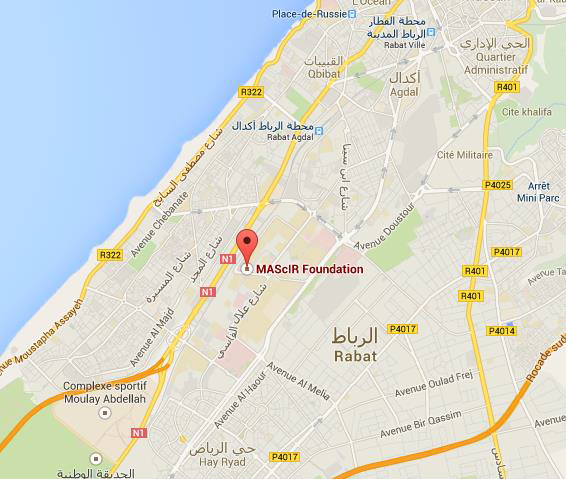
\includegraphics[width=0.75\textwidth]{mascir_map}
\caption{Localisation de la fondation MAScIR}
\end{figure}

Rassemblant d’éminents chercheurs des quatre coins du monde, MAScIR regroupe des équipes scientifiques œuvrant dans des domaines innovants et complémentaires et met à leur disposition une infrastructure scientifique de pointe.\\

Initialement fondée en 2007 par le Gouvernement Marocain en tant que fondation à but non lucratif MAScIR a continué son expansion en créant :

\begin{description}
\item[MAScIR MicroElectronics] a pour objectif de devenir un centre de Recherche et Développement dans le domaine de la microélectronique.
\item[MAScIR BioTechnology] deuxième centre inscrit dans MAScIR œuvrant dans le domaine de la biotechnologie : recherche et développement des médicaments ou des biocides.
\item[NanoTechnology] qui a pour mission de mener des recherches appliquées, innovantes et à la fine pointe de la technologie dans le domaine des nanomatériaux et des nanotechnologies. Ces recherches sont menées par une équipe internationale de haut calibre travaillant dans un environnement unique et utilisant une infrastructure de pointe.
\end{description}

\subsection{Partenaires de la foundation}
Les principaux partenaires de la fondation MASCIR MicroElectronics sont :
\begin{description}
\item[Lear Corporation] est l’un des principaux fournisseurs mondiaux de sièges automobiles et les systèmes de gestion de l’énergie électrique.
\item[Thales] figure parmi les leaders européens de la fabrication et de la commercialisation d'équipements et de systèmes électroniques destinés aux secteurs de l'aérospatial, du transport, de la défense et de la sécurité.
\item[OCP] est un acteur incontournable sur le marché des phosphates et de ses produits dérivés. Présent sur toute la chaine de valeur, il est le premier exportateur de cette matière dans le monde.
\item[COSUMAR] est un groupe marocain, filiale de la Société nationale d'investissement, spécialisé dans l'extraction, le raffinage et le conditionnement du sucre sous différentes formes. Il est devenu l'unique opérateur sucrier marocain après l'acquisition de SUTA, SUCRAFOR, SUNABEL et SURAC en 2005.
\item[STERIMED] est une société spécialisée dans le domaine de l’eau et des technologies de l’environnement. Son objectif est d’accompagner les entreprises et collectivités dans la résolution des problématiques liées à l’eau, l’environnement.
\end{description}

\subsection{Structure et hiérarchie}
La Fondation est gérée par un conseil d’administration qui est investi de pouvoirs de gestion à cet égard. Le Conseil dispose de quatre comités distincts : un Comité d’Investissement, un Comité de suivi, un comité de vérification et un Comité de Rémunération; qui assurent une gestion rapprochée des sujets relatifs à leur mission.
\begin{description}
\item[Conseil d'administration] détermine les orientations stratégiques de MAScIR et veille à leur mise en œuvre dans des réunions régulières. En prenant des décisions, le Conseil compte sur le travail des comités spécialisés.
\item[Comité de vérification] le rôle principal du Comité d'audit est de permettre à la Commission de veiller à la qualité des contrôles internes et l'intégrité de l'information divulguée aux intervenants et aux partenaires.
\item[Comité des Rémunérations] est responsable de faire des recommandations au Conseil sur la nomination des administrateurs. Il est également responsable de l'examen de la politique en matière de rémunération de la haute direction au sein de MAScIR.
\item[Comité de suivi] surveille la mise en œuvre effective et correcte des projets dans le cadre de l'accord signé entre MAScIR et le Gouvernement marocain.
\item[Comité d'Investissement] assiste le Conseil d'administration dans l'accomplissement de sa responsabilité de surveillance pour les actifs d'investissement liés à l'équipement scientifique.
\end{description}

\section{Présentation du département microélectronique}
MAScIR Micro est un centre d’innovation et développement de technologie dans le domaine de la microélectronique. Il se focalise sur la simulation, les tests, le design, le packaging, la qualification et le prototypage des produits microélectroniques.
\subsection{Mission}
Le programme Microélectronique a réuni une équipe de direction de classe mondiale pour assurer la traction initiale sous licence des technologies de pointe qui sont disponibles pour une utilisation immédiate. \\

Le programme Microélectronique a réuni une équipe de direction de classe mondiale pour assurer la traction initiale sous licence des technologies de pointe qui sont disponibles pour une utilisation immédiate. \\

MAScIR Micro fournit des services pour des clients industriels, mais elle développe aussi son propre business dans les domaines suivants :
\begin{itemize}
\item L’intégration et la miniaturisation des systèmes microélectroniques.
\item L’analyse de fiabilité et défaillance des produits.
\item Modélisation des systèmes complexes.
\item Prototypage et industrialisation des produits innovants.
\item Industrialisation des idées et résultats académiques.
\end{itemize}

\subsection{Laboratoires}
Le département microélectronique de MAScIR possède plusieurs laboratoires équipés de technologie avancée :
\begin{itemize}
\item Salle blanche
\item Laboratoire de fiabilité et analyse de défauts
\item Laboratoire électronique
\end{itemize}

\begin{figure}[H]
\centering
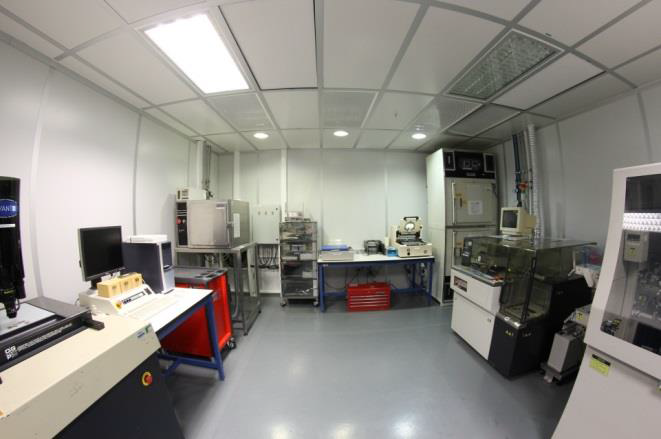
\includegraphics[width=0.75\textwidth]{cleanroom}
\caption{Salle blanche}
\end{figure}

\begin{figure}[H]
\centering
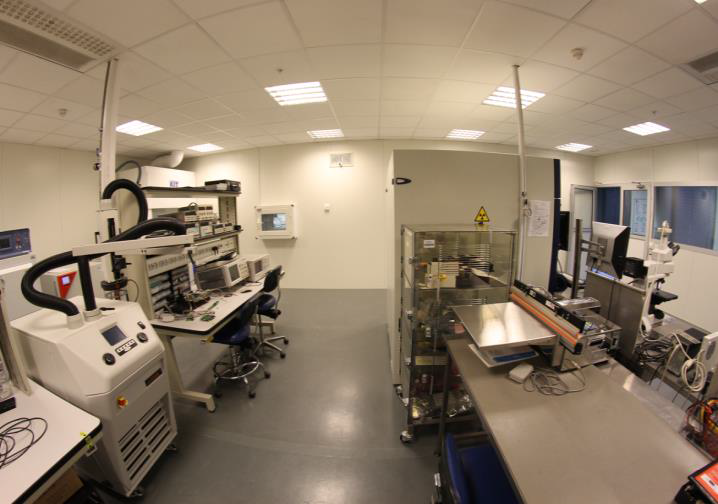
\includegraphics[width=0.75\textwidth]{labo}
\caption{Laboratoire de fiabilité et analyse de défauts}
\end{figure}

\subsection{Équipements}
\begin{itemize}
\item Ligne CSP (Chip Scaled Packaging)
\item Ligne SMT (Surface Mount Technology)
\item SAM (Scanning Accoustic Microscope)
\item X-Ray
\item Chambres climatiques
\end{itemize}

Pour plus d'informations, visiter le site de l'entreprise : \texttt{http://www.mascir.ma}.

\section{Description et déroulement du stage}
\subsection{Activités exercées}
Durant ce stage de fin d’études, j’ai eu l’opportunité de côtoyer le monde industriel et plus précisément de la microélectronique ce qui m’a permis d’assister et participer à plusieurs missions et projets que ce soit au sein de MAScIR ou à l’extérieur.\\

Mis à part le travail sur mon projet, j’ai pu suivre le processus du packaging allant du découpage wafer au marquage boitier et sciage.\\

Parallèlement, J’ai assisté à des manœuvres de vérification de qualité des produits livrés à MAScIR.\\

Par ailleurs, j’ai pu bénéficier d’un encadrement étroit en préparant des réunions pour garantir un bon état d’avancement du projet.

\subsection{Répartition des tâches}
%you need to revise mistakes
\noindent
\textsc{1\textsuperscript{ère} et 2\textsuperscript{ème} semaines :}
\begin{itemize}
\item Visite du local et réunions pour cerner le projet.
\item Bibliographie sur les system RFID.
\end{itemize}
\textsc{3\textsuperscript{ème} et 4\textsuperscript{ème} semaines :}
\begin{itemize}
\item Etude du marcher et choix des tags et lecteur rfid.
\item Participer à la résolution des problèmes du lecteur existant.
\end{itemize}
\textsc{5\textsuperscript{ème} et 6\textsuperscript{ème} semaine :}
\begin{itemize}
\item Etude et familiarisation avec le language \emph{.NET C\#}
\item Realisation d'un prototype de test de lecture de tages.
\end{itemize}
\textsc{7\textsuperscript{ème} et 8\textsuperscript{ème} semaine :}
\begin{itemize}
\item Proposition d'algorithme d'amelioration des performance de la commincation client-lecteur
\item Implementation final du prototype du nouveau protocol de communiation client lecteur.
\end{itemize}
\textsc{9\textsuperscript{ème} semaine :}
\begin{itemize}
\item Developpement d'une interface utilisateur pour le control du flux des donnee et gestion de stockage.
\item Etude du marcher marcaine de l'agrigulture et Etude de besoin .
\end{itemize}
\textsc{10\textsuperscript{ème} et 11\textsuperscript{ème} semaine :}
\begin{itemize}
\item Developpement de la Version une de l'application SmartFlah.
\item Amelioration de la version une de l'application SmartFlah
\end{itemize}
\textsc{12\textsuperscript{ème} et 13\textsuperscript{ème} semaine :}
\begin{itemize}
\item Etude Profondis sur les Tag RFID UHF.
\item Realisation du 1er prototype d'antenne UHF RFID
\end{itemize}
\textsc{14\textsuperscript{ème} et 15\textsuperscript{ème} semaine :}
\begin{itemize}
\item Etude des methode d'optimisation du tailet performance d'antenne.
\item simulation sur CST du 2eme prototype d'antenne
\end{itemize}
\textsc{16\textsuperscript{ème} et 17\textsuperscript{ème} semaine :}
\begin{itemize}
\item simulation sur CST du 3eme prototype d'antenne
\item Redaction du rapport
\end{itemize}



\chapter{Contexte Général du projet}
Le but de ce chapitre est de présenter la problématique du projet, le cahier des charges, la démarche suivie pour répondre au besoin de l’ensemble des parties prenantes du projet et le plan d’action.
\section{Cahier des charges}
\subsection{Objectif}
L’objectif de ce projet est l'étude et la réalisation d’une solution RFID UHF qui assure l’identification et la traçabilité des entrées et sorties des palettes. Choisire les tags adaptés aux besoins en respectant les conditions d’utilisation et type de lecteur et de développer un logiciel de gestion des palettes. 
Et comme deuxième axe,la réalisation d’un transpondeur RFID UHF et une application Android pour gestion du secteur d'agriculture qui permet a
l’utilisateur de profiter des fonctions offerte par le système à distance. \\
\subsection{Cachier des charges}
Assurer l’identification et la traçabilité des entrées / sorties palettes
\begin{itemize}
\item Choix des puces/tags adaptés aux besoins (conditions d’utilisation et type de lecteur).
\item Établir un programme de gestion des palettes en assurant la traçabilité de leur mouvement.
\item Réalisation et test d’un prototype.\\
\end{itemize}
\subsection{Mise au point de la problématique}
Ce projet consiste à développer un système de traçabilité des entrées et sorties des palettes. Trouver les causes racines, choisir les solutions optimales pour un problème ou une situation nécessite une grande compréhension du problème. Dans ce sens, la méthode QQOQCP permet d'avoir des informations élémentaires suffisantes sur toutes les dimensions du problème, pour identifier ses aspects essentiels.\\\\\\\
        
\begin{longtable}{|l|c|}
  \hline
  Quoi & Activité : Développement d’un un système de traçabilité \\
       &  Produit : logiciel , Application Android, Tag UHF \\
  \hline
  Qui & Division : Client MAcIR\\
  \hline
  Où & MAcIR\\
  \hline
  Quand & Du 15/02/2016 au 15/06/2015\\
  \hline
  Comment & État d’art sur les techniques RFID \\
          &  existantes afin de développer un autre plus adapté.\\
  \hline
  Pourquoi & Fournir un système de traçabilité des entrées et sorties des palettes.\\
  \hline
  
\caption{QQOQCP}
\end{longtable}

\section{Déroulement chronologique du stage}
Durant les 4 mois de mon stage, les tâches relatives à mon projet de stage sont organisé de la façon suivante:
\subsection{Etapes	de	réalisaion}
\begin{longtable}{|p{0.35\textwidth}|p{0.2\textwidth}|p{0.2\textwidth}| p{0.15\textwidth}|}
\hline
\textbf{Tâche} & \textbf{Date de début} & \textbf{Date de fin} & \textbf{Durée} \\
\hline
Visites et réunions & 16/02/16 & 18/02/16 & 3 jours \\
\hline
Bibliographie RFID & 15/02/16 & 26/02/16 & 10 jours \\
\hline
Étude du marcher et choix des tags et lecteur RFID & 29/02/16 & 04/03/16 & 5 jours \\
\hline
Participer à  la résolution des problèmes du lecteur existant.
 & 07/03/16 & 11/03/16 & 5 jours \\
\hline
Étude et familiarisation avec le langage \emph{.NET C\#} & 14/03/16 & 18/03/15 & 5 jours \\
\hline
Réalisation d'un prototype de test de lecture de tags & 14/03/15 & 25/03/15 & 10 jours \\
\hline
 Étude et proposition d'algorithme pour amélioration des performance de la communication client-lecteur
 & 28/03/16 & 30/03/16 & 3 jours \\
\hline
Implémentation final du prototype du nouveau protocole de communication client lecteur.
 & 30/03/16 & 10/04/16 & 11 jours \\
\hline
Développement d'une interface utilisateur pour le contrôle du flux des données et gestion de stockage.
 & 11/04/16 & 19/04/16 & 7 jours \\
\hline
Étude du marcher marocaine de l'agriculture et Étude de besoin & 20/04/16 & 22/04/16 & 3 jours \\
\hline
Développement de la Version une de l'application SmartFlah. & 20/04/16 & 25/04/16 & 5 jours \\
\hline
Étude Approfondis sur les Tag RFID UHF  & 25/04/16 & 28/04/16 & 4 jours \\
\hline
Prestation de MAsIR a SIAM  & 29/04/16 & 29/04/16 & 1 jours \\
\hline
Amélioration de la version une de l'application SmartFlah & 02/05/16 & 04/05/15 & 3 jours \\
\hline
Réalisation du 1 er prototype d'antenne UHF RFID & 05/05/16 & 13/05/16 & 7 jours \\
\hline
Étude des méthode d'optimisation du taille et performance d'antenne. & 16/05/16 & 20/05/16 & 2 jours \\
\hline
simulation sur CST du 2 ème et 3 ème prototype d'antenne & 23/06/16 & 10/06/16 & 15 jours \\
\hline
Rédaction du rapport & 11/06/16 & 15/06/16 & 4 jours \\
\hline
\caption{Répartition des tâches}
\end{longtable}
\subsection{Diagrammes	de	Gantt}
figures...
\section{Décomposition du projet}
Le projet est décomposé principalement en 3 parties :
\begin{itemize}
\item Développement du Middleware et de l'interface graphique: une partie qui consiste a assurer la communication entre le serveur et le lecteur RFID.
\item Développement de l'application SmartFlah pour la gestion des tags animal.
\item Le transpondeur : la conception du transpondeur UHF RFID de petite taille.\\
\end{itemize}

Chaque partie sera étudiée indépendamment dans les chapitres qui suivent.

\chapter{Etude	détaillée du Projet}
RFID ou identification par fréquence radio, est une technologie en croissance rapide qui a le potentiel de faire de grands impacts économiques sur de nombreuses industries. Bien que la RFID est une technologie relativement ancienne, les progrès les plus récents dans la technologie de fabrication de puces RFID font pratique pour de nouvelles applications et paramètres.\\
Ce chapitre est dédié a l'étude	 détaillée de la solution RFID.
\section{Description de la solution}
Cette section présente les bases des systèmes RFID et offre la taxonomie des différents types de systèmes RFID. Nous discutons brièvement deux normes RFID majeures et comment ils se rapportent à la pratique.
\subsection{Le system de base RFID}
La discussion de la technologie RFID a tendance à se concentrer uniquement sur les étiquettes. Il est plus exact de voir RFID comme un système complet qui comprend non seulement des étiquettes, mais aussi d'autres éléments importants. Les systèmes RFID sont constitués d'au moins trois composants principaux:
\begin{itemize}
\item Les étiquettes RFID ou transpondeurs, qui transportent des données d'objet d'identification.
\item Lecteurs RFID, ou des émetteurs-récepteurs, lire et écrire des données dans l'étiquette.
\item Bases de données associés pour l'enregistrement de la donnée d'identification\\
\end{itemize}

Nous illustrons l'interaction de ces composants dans la figure 3.1. Sur cette figure, trois étiquettes sont lisibles par un ou les deux lecteurs, A et B. Par exemple, l'étiquette 1 est lisible que par A, tandis que l'étiquette 2 est lisible par A et B, peut-être en raison de restrictions l'accès. Les lecteurs peuvent alors se connecter à des bases de données avec des enregistrements associés à des données d'identification. Dans ce cas, deux bases de données ont chacun leur propre record.\\
\begin{figure}[H]
\centering
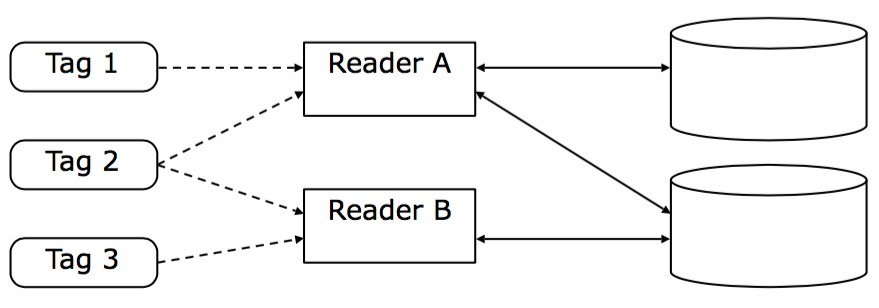
\includegraphics[width=\textwidth]{shema}
\caption{Illustration du système RFID}
\end{figure}
\subsection{Les composants essential d'un system RFID}
\subsubsection{Les tags}
Les tags sont attachés à tous les objets à identifier dans un système RFID. Un tag est généralement
composé d'une antenne ou un élément de couplage, et un circuit intégré. Un important
distinction qui sera discuté plus tard est la source d'alimentation d'un tag. Souvent, les étiquettes ne portent pas une source d'alimentation et doit passivement récolter toute l'énergie d'un signal RF.

Il existe plusieurs types de tags qui offrent des fonctionnalités différentes, ont des puissances différentes
de sources ou fonctionnent à des fréquences radio différentes. Chacune de ces variables permet de déterminer
quelles applications une étiquette particulière peut être approprié. Ces différences seront examinées plus loin dans ce chapitre.

Les étiquettes modernes ont tendance à mettre en œuvre la fonctionnalité d'identification sur un circuit intégré (IC) qui
assure le calcul et le stockage. Dans le procédé de fabrication, ce circuit intégré est fixé ou
"Attaché" à une antenne avant d'être emballés dans un facteur de forme, comme une capsule de verre ou d'une feuille, qui est intégré dans un produit final.Dans la pratique, les différents fournisseurs effectuent souvent chacune de ces étapes de fabrication. Autres RFID
dessins peuvent être «chipless» ou avoir des informations d'identification au moment de la fabrication, à savoir
"Écriture une fois, lecture nombreuse". \\
\begin{figure}[H]
\centering
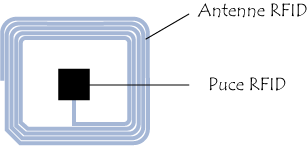
\includegraphics[height=3cm]{tag}
\caption{Tag RFID}
\end{figure}
\subsubsection{Reader/Lecteur}
Les lecteurs RFID communiquent avec des tag à travers un canal RF pour obtenir l'identification
. Selon le type de l'étiquette, cette communication peut être un simple ping ou peut être un protocole plus complexe de caractère multi-tour. Dans les environnements avec de nombreux points, un lecteur peut avoir à effectuer une algorithme d'anti-collision pour veiller à ce que les conflits ne peuvent pas se produire. Les protocoles anti-collision permettent aux lecteurs de communiquer rapidement avec beaucoup de tags en série.

Les lecteurs alimentent souvent ce que l'on appelle les étiquettes passives à travers leur canal de communication RF.
Ces types d'étiquettes ne portent aucune puissance à bord et comptent uniquement sur un lecteur pour fonctionner. Étant donné que ces tag sont si limitées, il compter sur un lecteur pour effectuer des calculs.
Les lecteurs se présentent sous plusieurs formes, fonctionnent sur de nombreuses fréquences différentes, et peuvent offrir un large éventail de fonctionnalités. Les lecteurs peuvent avoir leur propre puissance de traitement et de stockage interne, et peuvent offrir une connectivité réseau. Les lecteurs pourraient être une simple conduit à un système externe, ou pourraient stocker toutes les données pertinentes au niveau local.

À l'heure actuelle, de nombreuses applications reposent sur des dispositifs de lecture fixes. Les premiers essais de EPC à une grande chaîne de supermarchés intégrés dans les lecteurs entrées accueil baies fixes. Ces lecteurs scannent les étiquettes au niveau de la palette que les livraisons de produits arrivent. 

Les lecteurs RFID peuvent également être intégrés dans des appareils mobiles portatifs. Ces lecteurs mobiles permettraient à quelqu'un, par exemple, faire l'inventaire d'un entrepôt en marchant à travers ses allées. Le fabricant de téléphone cellulaire Nokia propose déjà des fonctionnalités RFID de lecture dans certains de leurs téléphones cellulaires. les balises de type EPC deviennent très réussie, intéressante et les applications grand public utiles pourraient se poser. Si cela se produit, la fonctionnalité de lecture RFID pourrait devenir une caractéristique commune sur les téléphones, PDA, ou d'autres dispositifs informatiques portables cellulaires.
\begin{figure}[H]
\centering
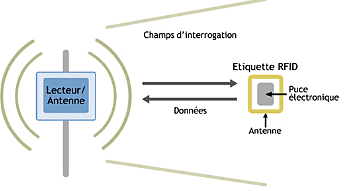
\includegraphics[height=4cm]{reader}
\caption{Interaction du Lecteur RFID avec son environnement}
\end{figure}
\subsubsection{La bases de donnée}
bases de données RFID associent l'identifiant de tag avec un enregistrements. Ces enregistrements peuvent contenir des informations sur les produits, les journaux de suivi, les données de ventes, ou les dates d'expiration. Des bases de données indépendantes peuvent être construites tout au long de la chaîne d'approvisionnement par des utilisateurs indépendants, ou peuvent être intégrés dans un système de base de données centralisée ou fédérée.\\

Les bases de données sont supposées avoir une connexion sécurisée aux lecteurs. Bien qu'il existe des scénarios où les lecteurs peuvent ne pas être dignes de confiance, il est souvent utile de faire écrouler les notions de lecteur et la base de données en une seule entité. Par exemple, si les étiquettes contiennent toutes les informations de produits en cause, il n'y a pas besoin de faire un appel à une base de données hors site.

On peut imaginer un système fédéré de bases de données back-end, où chaque fabricant de produit conserve son propre service de consultation produit. Dans ces paramètres, il peut être utile de déployer un (ONS) \footnote{service Object Naming} pour localiser les bases de données associées à une valeur d'identification d'étiquette. Un ONS permet au lecteur de trouver un ensemble de bases de données associées à une valeur d'identification d'étiquette particulière. Ceci est analogue à l'Internet avec le (DNS) \footnote{Domain Naming Service} qui renvoie les adresses des serveurs de noms qui peuvent traduire les noms de domaine en adresses IP numériques. ONS n'a pas encore été largement adopté dans la pratique.
\subsection{Source d'énergie d'un Tag}
Comme brièvement mentionné précédemment, les étiquettes peuvent obtenir leur pouvoir de plusieurs manières différentes. La source d'énergie est une propriété essentielle d'une étiquette, car il va déterminer la distance de lecture potentielle d'une balise, la durée de vie, le coût, et quel genre de fonctionnalités qu'il peut offrir. La source d'énergie sera également important pour déterminer comment une étiquette peut être orienté et quelles formes physiques qu'il peut prendre.Il existe trois catégories principales de sources d'énergie de tag: actifs, semi-passifs, et passifs.\\

 Les étiquettes actives ont leur propre source d'énergie, telle qu'une batterie, et peuvent initier une communication à un lecteur ou d'autres balises actives. Parce qu'ils contiennent leur propre source d'alimentation, les étiquettes actives ont généralement une plage de fonctionnement beaucoup plus large que passifs-tags. Une caractéristique clé de balises actives est qu'ils sont en mesure de lancer leur propre communication avec les lecteurs. Les balises actives avancées, pourraient même former des réseaux ad hoc les uns avec les autres. Une application utile est les balises actives dans des conteneurs d'expédition , qui peuvent tomber hors navires sur les mers agitées. Ces conteneurs manquants parfois ne sont pas reconnus jusqu'à ce que le navire à quai . Une étiquette à puce avec un capteur accéléromètre pouvait détecter quand il est tombé et distribuer un journal de sa disparition avant de sombrer dans l'océan.\\

Par contre, un semi-passif (ou semi-actif) tag ont une batterie interne, mais ne sont pas en mesure d'initier des communications. Cela garantit que les étiquettes semi-passives ne sont actives que lorsqu'il est interrogé par un lecteur. Parce que les étiquettes semi-passives ont une source d'énergie interne, ils offrent une lecteur plus large que les passives, mais à un coût plus élevé.\\


Un exemple d'application qui utilise souvent des étiquettes semi-passives est \emph {tollbooths} électroniques. les étiquettes passives sont généralement collée à l'intérieur du pare-brise d'une voiture. Lorsque la voiture passe par un péage, il lancera une requête à l'étiquette et lire un compte identifiant de l'étiquette. La batterie de bord permet la balise être lues à une distance considérable. Cependant, étant donné que l'étiquette ne doit diffuser lorsqu'il est interrogé, il peut rester inactif la plupart du temps et économiser de l'énergie. Les étiquettes semi-passives sont également souvent utilisés dans les palettes au niveau de suivi ou de suivi des composants tels que des pièces d'automobile lors de la fabrication.\\


Les étiquettes passives ont ni leur propre source d'énergie, ni la capacité d'initier la communication. Les étiquettes passives obtiennent de l'énergie par la récolte à partir d'un signal de communication RF entrant. À des fréquences plus basses, cette énergie est typiquement récoltées par induction, tandis qu'à des fréquences plus élevées, il est récolté par capacité.\\

Bien que les étiquettes passives ont la plus courte distance de lecture de tous les trois types alimentant, ils sont les moins chers à fabriquer et plus facile à intégrer dans des produits. Les batteries sont relativement coûteux et ne peuvent pas facilement être incorporés dans certains articles, comme les emballages en papier. Pour cette raison, les étiquettes passives sont des balises les plus courantes.\\

En l'absence d'une source d'énergie interne dicte de nombreuses propriétés des étiquettes passives. D'abord, ils ne peuvent pas fonctionner sans la présence d'un lecteur, bien que étiquette passive pourrait temporairement en cache un peu d'énergie dans un condensateur. En raison de leur faible nécessairement signal de réponse, les étiquettes passives sont souvent plus sensibles au bruit ambiant ou des interférences. Le tableau 1 compare diverses propriétés des étiquettes passives, semi-passives et actives.\\

\begin{longtable}{|p{0.35\textwidth}|p{0.2\textwidth}|p{0.2\textwidth}| p{0.15\textwidth}| p{0.15\textwidth}|}
\hline
\textbf{Type} & \textbf{Passif} & \textbf{Semi-Passif} & \textbf{Active} \\
\hline
\textbf{Source d'énergie} & énergie récolté du RF & Batterie & Batterie \\
\hline
\textbf{Communication} & Réponse seulement & Réponse seulement & Répondre ou initier \\
\hline
\textbf{Max Range} & 10 M & 100 M &  100 M \\
\hline
\textbf{Coût relatif} & Le moins cher & Plus cher & Très cher \\
\hline
\textbf{Exemple Applications} & EPC cartes de proximité & télé péage &  \emph {Livestock tracking} \\
\hline
\caption{Comparaison de tag passif , semi- passif et actif}
\end{longtable}


\subsection{Fréquences de fonctionnement}
Les systèmes RFID a une variété de fréquences radio. Chaque bande de fréquences offre sa propre avantage d'exploitation, les exigences de puissance et de performance. Différentes gammes peuvent être soumis à des règlements ou des restrictions qui limitent ce que les applications peuvent être utilisés pour.
Les métaux et les liquides présentent généralement le plus gros problème dans la pratique. En particulier, les balises actives dans l'ultra-haute fréquence (UHF) ne fonctionnent pas correctement à proximité de liquides ou de métal.\\


Fréquence de fonctionnement est également important dans la détermination des dimensions physiques d'une étiquette RFID. Différentes tailles et formes des antennes fonctionnent à des fréquences différentes. La fréquence de fonctionnement détermine également la possibilité d'interagir physiquement avec les autres. Par exemple, l'empilage des étiquettes plates feuille d'incrustation sur le dessus de l'autre peut interférer ou empêcher les balises de la lecture correctement. Le tableau 2 énumère les fréquences standard et leurs distances de lecture passifs respectifs.\\
\begin{longtable}{|p{0.35\textwidth}|p{0.2\textwidth}|p{0.2\textwidth}|}
\hline
\textbf{Gamme de fréquences} & \textbf{fréquences} & \textbf{Distance de lecture} \\
\hline
Basse fréquence & 120-140 KHz & 10-20 cm  \\
\hline
Haute Fréquence (HF) & 13,56 MHz & 10-20 cm \\
\hline
Ultra-haute fréquence (UHF) & 868-928 MHz & 3 mètres \\
\hline
Micro onde & 2,45 et 5,8 GHz & 3 mètres \\
\hline
Ultra-Wideband (UWB) & 3,1-10,6 GHz & 10 m \\
\hline
\caption{fréquences de fonctionnement RFID}
\end{longtable}
\subsubsection{Basse fréquence (LF)}
Basse fréquence (LF) étiquettes RFID fonctionnent généralement dans la gamme 120-140 kilohertz. Le plus souvent, les balises LF sont passivement alimentés par induction. En conséquence, ils ont généralement de très courts intervalles de lecture 10-20 centimètres.\\

Les balises LF peuvent être utilisés dans des environnements difficiles et peuvent fonctionner à proximité de métal, des liquides, ou de la saleté. Cela les rend utiles pour des applications comme les étiquettes d'identification pour animaux de compagnie implantables ou des étiquettes de gestion de blanchisserie. Un inconvénient de balises LF est qu'ils ont une très faible taux de lecture de données par rapport à d'autres fréquences de fonctionnement.\\

LF balises sont souvent utilisés dans les systèmes d'immobilisation de la voiture et de contrôle d'accès. Dans ces systèmes, une voiture ne démarre que si une balise de LF, généralement attaché à la clé de contact, est à proximité de l'allumage. Cela prend avantage de courte portée de lecture de LF et l'utilise comme un élément de sécurité.\\

En 20016, LF étiquettes passives peuvent être achetés en vrac pour 10 DH par tag ou moins. Deux grands fabricants de balises LF sont Texas Instruments et Phillips Semiconductor. La norme \emph{ISO 18000-2 standard} offre des spécifications pour les étiquettes RFID LF.

\subsubsection{Haute fréquence}
Haute fréquence (HF) étiquettes RFID fonctionnent à la fréquence de 13,56 MHz. étiquettes HF sont souvent emballés dans un facteur d'incrustation de feuille ou sous forme de carte de crédit. Cela rend les balises HF utiles pour la construction de contrôle d'accès, les cartes de crédit sans contact, et des badges d'identification. Encore une fois.\\

Les étiquettes HF sont également utilisés dans de nombreuses applications de suivi. Les bibliothèques et les librairies utilisent souvent HF incrustations de feuilles pour suivre les livres. Certains aéroports ont commencé à utiliser HF RFID étiquettes à bagages pour les applications de manutention de bagages.\\

les étiquettes HF offrent un taux de lecture de données plus élevé que les balises LF, mais ne réussissent pas aussi bien que les balises de LF à proximité de métaux ou de liquides. balises HF font, cependant, offrent de meilleures performances à proximité de métaux ou de liquides que les tags UHF font.\\

La gamme de fréquence HF se trouve sur une partie fortement réglementée du spectre radio. Les signaux transmis par les lecteurs doivent fonctionner dans une bande de fréquence étroite. Cela pose un problème pour les environnements électroniques sensibles, tels que les équipements médicaux, qui fonctionnent sur des fréquences voisines. Cela rend les balises HF inappropriée pour les environnements comme les hôpitaux.\\

En 2016, HF étiquettes passives peuvent être achetés pour 5DH ou moins par étiquette en quantité. Texas Instruments et Phillips offrent tous deux lignes tag HF, bien qu'il existe de nombreux fabricants plus petits et spécialisés ou intégrateurs dans l'espace de HF.
Organisation internationale de normalisation (ISO) spécifications pour les étiquettes RFID HF sont spécifiées par la norme \emph{ISO 18000-3 norme} [11]. spécifications connexes HF sans contact des cartes à puce et les cartes de proximité apparaissent dans les normes ISO 14443 [9] et 15693.
\subsubsection{Ultra-haute fréquence}
Ultra-haute fréquence (UHF) étiquettes RFID fonctionnent dans la gamme de 868 à 928 mégahertz. balises européennes fonctionnent généralement dans la gamme 868-870 MHz, tandis que les États-Unis et au Canada fonctionnent à 902-928 MHz. tags UHF sont les plus couramment utilisés pour les applications de suivi et de gestion de la chaîne logistique article. Ceci est en grande partie parce qu'ils offrent une gamme plus lu et sont moins chers à fabriquer en vrac que LF ou HF tags. Les étiquettes EPC de première génération fonctionnent à des fréquences UHF.\\

Un inconvénient majeur de tags UHF est qu'ils éprouvent des interférences à proximité de liquides ou de métaux. De nombreuses applications telles que le suivi des animaux, suivi des conteneurs en métal, ou même de nombreux systèmes de contrôle d'accès sont irréalisables avec des étiquettes UHF. Certains matériaux ont été développés qui peuvent protéger les tags UHF de distorsion liés à métal, mais ceux-ci peuvent être coûts prohibitifs à utiliser dans la pratique. lecteurs UHF peuvent également interférer avec l'électronique sensible comme l'équipement médical.\\

tags UHF sont une technologie relativement récente que LF ou HF, et les coûts de lecteur sont généralement plus élevés que les lecteurs de LF faible largeur de bande. En 2016, les tags UHF peuvent être achetés en quantités pour moins de 1DH par étiquette passive. étiquettes UHF coûts aussi bas  0.5DH sont susceptibles d'arriver sur le marché dans les prochaines années. Spécifications pour les étiquettes RFID fonctionnant à des fréquences UHF sont définies à la fois par l'ISO 18000-6 et à la norme EPCGlobal .
\subsubsection{Micro-ondes} 
étiquettes de micro-ondes fonctionnent soit à 2,45 ou 5,8 GHz. Cette gamme de fréquences est parfois appelée fréquences de super-haute (SHF). La technologie RFID de micro-ondes est entré en usage assez récemment et se développe rapidement. étiquettes à micro-ondes utilisées dans la pratique sont généralement semi-passif ou actif, mais peuvent aussi se présenter sous forme passive. balises à micro-ondes semi-passives sont souvent utilisés dans l'identification de la flotte et des applications de télé-péage.\\


Les systèmes à micro-ondes offrent plus les taux de lecture que UHF et gammes équivalentes de lecture passive. Plages de lecture semi-passives et actives des systèmes de micro-ondes sont souvent plus grandes que leurs homologues UHF. Certains micro-ondes balises actives peuvent être lues à partir des distances allant jusqu'à 30 mètres, ce qui est moins de tags UHF comparables. Cependant, les implémentations physiques des micro-ondes étiquettes RFID peuvent être beaucoup plus petit et compact que basse fréquence des étiquettes RFID.\\


Il y a plusieurs inconvénients à des balises à micro-ondes. La première est qu'ils consomment relativement plus d'énergie que leurs homologues de fréquence inférieure. étiquettes de micro-ondes sont généralement plus chers que les tags UHF. Commercialement balises actives disponibles coûtent autant que 250 DH par tag en 2016.
Un autre problème est que le sans fil 802.11b / g réseaux (WiFi) peuvent interférer avec les systèmes micro-ondes RFID. Dispositifs d'application de la ZigBee 802.15 prochaine norme sans fil pourraient potentiellement entrer en conflit avec des dispositifs micro-ondes RFID ainsi.
L'ISO 18000-4 et ISO 18000-5 rejeté [11] Les normes offrent des spécifications respectives pour 2,45 et 5,8 gigahertz étiquettes RFID.
\subsubsection{Ultra-Wideband}
Ultra-wideband (UWB) appliquée à la RFID est assez récente. Plutôt que d'envoyer un signal fort sur une fréquence particulière, UWB utilise des signaux de faible puissance sur une très large gamme de fréquences. Le signal sur une fréquence particulière utilisée par UWB est très faible, mais dans l'ensemble, la communication est assez robuste. Dans la pratique, certaines implémentations de UWB fonctionnent de 3,1 à 10,6 GHz.\\

Les avantages de l'UWB sont qu'il a une très longue portée en ligne de mire de lecture, peut-être 200 mètres dans certains contextes. UWB est également compatible avec le métal ou les liquides. Comme le signal sur une fréquence particulière est très faible, UWB ne pas interférer avec les équipements sensibles. Par conséquent, une application anticipée était suivi des actifs dans un milieu hospitalier.\\

Un inconvénient d'implémentations actuelles de UWB est qu'il doit être actif ou au moins semi-passive. Cependant, étant donné que les balises UWB diffusent des signaux très faibles, ils ont relativement faible consommation d'énergie. En 2006, il est difficile de savoir si la technologie existe pour créer un UWB tag passive.
La technologie RFID UWB est encore dans ses premières phases et il y a peu de produits disponibles dans le commerce. Les coûts de 50DH par tag en vrac sont raisonnables dans un proche avenir.
\subsection{Fonctionnalité}
La fonctionnalité RFID de base est l'identification. Lorsqu'il a été interrogé par un lecteur, les balises retournent un autre identificateur qui peut être utilisé pour récupérer d'autres enregistrements de données. Cependant, les étiquettes peuvent offrir d'autres fonctionnalités utiles dans différentes applications. Les principes et les technologies de ces différents types de balises sous-jacentes sont si étroitement liés aux étiquettes RFID strictes, qu'ils ont souvent collectivement appelés «RFID». Bien que pas strictement RFID, nous discutons de plusieurs classes majeures d'appareils liés à la RFID.\\

Nous avons partagé des étiquettes RFID de style en cinq grandes catégories: EAS, en lecture seule EPC, EPC, étiquettes de capteurs, et motes. Ceux-ci seront appelés classes A à E. EPCglobal propose cinq classes similaires de tag basé sur la fonctionnalité baptisée classe 0 à la classe 4 [6]. Les classes EPCglobal aligner étroitement avec les nôtres, mais diffèrent quelque peu. Ces cinq classes sont résumés dans le tableau 3.

\begin{longtable}{|p{0.1\textwidth}|p{0.2\textwidth}|p{0.2\textwidth}| p{0.15\textwidth}|p{0.2\textwidth}|}
\hline
\textbf{Classe} & \textbf{Nom} & \textbf{Mémoire} & \textbf{Source d'énergie} & \textbf{Caractéristi-ques} \\
\hline
A & EAS & Aucun & Passif & article surveillance \\
\hline
B & Lecture seule EPC & Lecture seulement & Passif & identification seulement \\
\hline
C & EPC & Lire et écrire & Passif & Enregistrement de données \\
\hline
D & capteur Balises & Lire écrire & Semi-passif & capteurs environnementaux \\
\hline
E & motes & Lire écrire & actif & Réseautage ad hoc \\
\hline
\caption{Classes de fonctionnalité des Tags}
\end{longtable}

\subsection{Normes}

Les deux normes RFID les plus pertinents sont l'Organisation internationale de la norme ISO / IEC 18000 de normalisation norme [11] et les normes de EPCglobal [6]. Ces normes ne sont pas en concurrence, et il est concevable que la norme EPCglobal pourrait éventuellement être adopté dans une norme ISO.
EPCglobal définit des spécifications pour les étiquettes de type EPC fonctionnant dans la gamme UHF.
La norme ISO 18000 a 6 parties d'adressage différentes gammes de fréquences:
\begin{itemize}
\item Partie 1 - Généralités normes
\item Partie 2 - LF
\item Partie 3 - HF
\item Partie 4 - Micro-ondes, 2,45 GHz
\item Partie 5 - Micro-ondes, 5,8 GHz
\item Partie 6 - UHF\\
\end{itemize}
\subsection{Modes de transfert d’énergie et de communication}
Dans ce premier cas ( figure 3.4) , l’onde RF se propageant de la base station vers le tag n’a pour but unique que de fournir de l’énergie au tag de façon à charger la  capacité d’alimentation  présente à son bord afin que celle-ci puisse être capable d’alimenter l’ensemble du tag pour assurer son bon fonctionnement. Aprés cette phase d'alimentation, le tag est apte à recevoir des ordres de commande provenant de la base station et de retourner des informations vers celle-ci. Puis le cycle recommence et il est à nouveau nécessaire de lui fournir de l'énergie pour continuer la communication et ainsi de suite. Bien évidemment, ceci prend du temps et manque parfois de souplesse.\\
\begin{figure}[H]
\centering
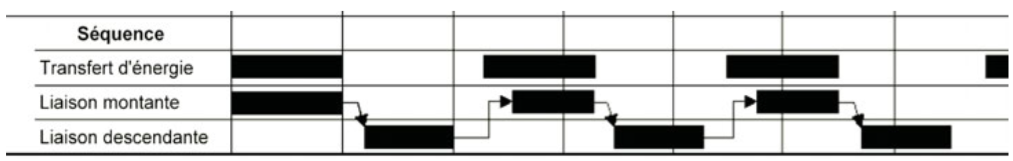
\includegraphics[width=\textwidth]{figa}
\caption{Mode de transfert d'énergie non simultané}
\end{figure}

Dans ce deuxième cas ( figure 3.5), au travers des principes et types de modulation utilisés, l'onde provenant de la base station est capable pendant la phase de l'échange base station vers tag d'assurer simultanément la fourniture de l'énergie et l'échange des informations (données).\\

\begin{figure}[H]
\centering
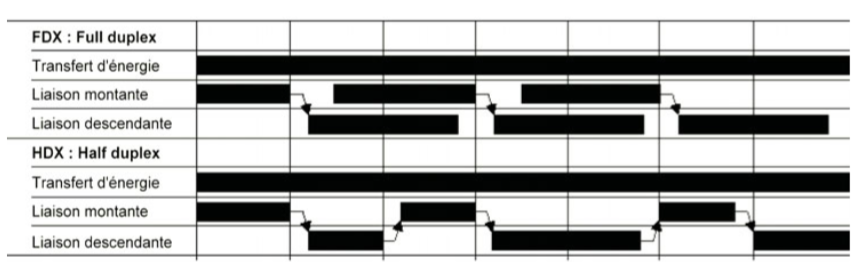
\includegraphics[width=\textwidth]{figb}
\caption{Mode de transfert d'énergie simultané}
\end{figure}

\begin{center}
\textbf{\emph{Note :}}\\
\emph{À noter que la trés grande majorité des tags du commerce fonctionnent selon ce dernier principe.}
\end{center}

\subsection{Liaison montante et liaison descendante}
Intéressons-nous d’abord aux échanges ayant lieu entre bases stations et tags. Ils sont de deux sortes et seront définis une fois pour toutes dans cet ouvrage de la manière suivante :
\begin{itemize}
\item de la base station vers le tag, dits liaison montante ;
\item du tag vers la base station, dits liaison descendante. \\
\end{itemize}
De plus afin d’éviter quelques problèmes de compréhension, quelle que soit l’intelligence embarquée dans le tag, nous supposerons que celui-ci ne fonctionne que sous des ordres commandes provenant de la base station. 
\subsubsection{Liaison montante ( forward link) de la base station vers le tag}
La liaison montante (de la base station vers le tag) a pour mission :
\begin{itemize}
\item d'assurer, si cela est possible, le transport de l'énergie vers le tag afin que celui-ci puisse assurer la taÌ‚che qui lui incombe ;
\item de servir de support à l'envoi de données de la base station vers le tag ;
\item d'assurer, si cela est possible, le transport de l'énergie vers le tag afin que celui-ci puisse assurer
\item dans le cas des systèmes fonctionnant en mode passif (voir définition un peu plus loin), lors de la phase de communication en liaison descendante, d'assurer la présence d'un support physique à la communication du tag vers la base station.\\
\end{itemize}

La communication montante est par principe assurée par un dispositif – la base station – qui émet une onde radiofréquence. Celle-ci est donc dotée d’un émetteur, un TRANSmitter. De par la présence de cet émetteur, la liaison montante est dite active. De plus, la base station comporte également à son bord un récepteur, un reCEIVER. La base station est donc un TRANSCEIVER. Dans le sens montant, la base station doit se faire comprendre par le tag au travers d’un co- dage numérique (binaire), d’un protocole de communication et d’un système de modulation de la fréquence porteuse ne devant pas ou peu affecter (le plus faiblement possible) la qualité d’une hypothétique télé-alimentation simultanée. Pour cela on peut employer des techniques de modulation de fréquence FSK \footnote{Frequency-Shift Keying}, ou encore de nombreuses méthodes de modulation d’amplitude ASK \footnote{Amplitude-Shift Keying}
\subsubsection{Liaison descendante de la modulation}
Contrairement à ce qu'on pourrait initialement penser, le transpondeur ne peut pas se comporter comme un émetteur de signaux RF. En effet, il ne dispose pas, dans son interface RF, des mécanismes permettant d'émettre un signal radio-fréquence vers la station de base.Les transpondeurs utilisent ce qu'on appelle la réflexion d'ondes pour se faire comprendre des lecteurs. \\

Pour cela, les tags utilisent une modulation différente que l'on nomme modulation de charge (Load Modulation) qui consiste à faire varier la charge résistive du circuit. Effectivement, en faisant varier la charge, le tag fait varier l'intensité du courant dans son circuit et donc l'intensité qui circule dans l'antenne. La consommation d'énergie qu'il représente dans le champ magnétique s'en trouve alors également modifiée et, par couplage magnétique, cela influe sur l'intensité du courant dans l'antenne de la station de base. De proche en proche, les signaux RF reçus de la station de base, qui sont réfléchis par le transpondeur, permettent donc de transporter des réponses en faisant varier l'intensité du circuit du lecteur.\\

Il s'agit ici d'un procédé assez complexe mais qui repose à la base sur de la modulation. Cette modulation de charge résistive à l'origine de la transmission de la réponse s'appuie sur une modulation courante appelée OOK \footnote{On Off Keying} et correspond à la modulation d'amplitude "tout ou rien". A l'aide d'une modulation de type OOK, comme présentée précédemment, on crée une modulation de charge qui fait varier la charge résistive du circuit et donc la tension aux bornes du circuit RF du transpondeur comme montré dans la figure 3.5.\\
\section{Le protocole de communication RFID}
Dans cette section je vais décrire le rôle de l'interface entre les lecteurs RFID et les clients. Dans ce qui suite sont les responsabilités de cette interface:
\begin{itemize}
\item Fournir des moyens pour commander un lecteur RFID  (lire les codes EPC sur les étiquettes), lire les étiquettes (lire d'autres données sur les étiquettes en dehors du code EPC), écrire dans les tags, et exécuter d'autres commandes d'accès protocole dépendant.
\item 
Fournir un moyen de rapporté l'état et la gestion des erreurs lors des opérations d'accès d'étiquette.
\item 
Fournir des moyens  nécessaires pour effectuer des commandes qui peuvent en avoir besoin, comme la commande 'Kill' dans le Protocole UHF Interface Air \cite{air}.
\item 
Fournir des moyens pour contrôler les aspects du fonctionnement du Protocole de Tag, y compris les paramètres de protocole et les paramètres de signalisation.
\item 
Fournir des moyens pour faciliter l'ajout du support pour les nouveaux protocoles d'air
\item 
Fournir des moyens pour la récupération des capacités de l'appareil lecteur.\\
\end{itemize}
\subsection{Rôle le d'interface}
L'infrastructure RFID est constituée des éléments de réseau qui participent à la gestion (par exemple, lecture / écriture / verrouillage) et la transmission de données de l'étiquette. La destination des données d'étiquette sont les éléments de réseau clients (applications par exemple, l'utilisateur final, base de données). Les éléments de réseau entre l'étiquette et les clients forment le support pour transporter les données de l'étiquette sur le réseau et de transmettre les commandes opérationnelles des balises.
\begin{figure}[H]
\centering
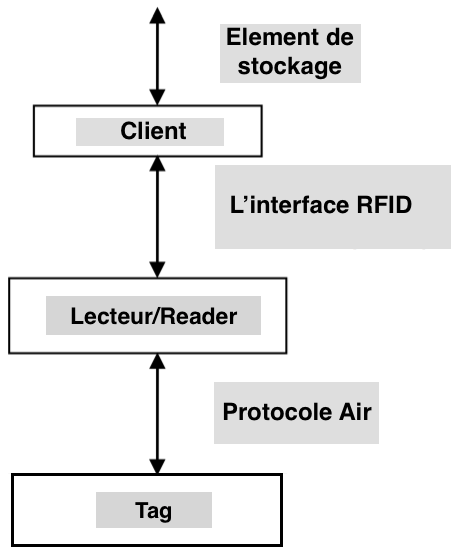
\includegraphics[width=6cm,height=8cm]{orga}
\caption{Organigramme de l'interface RFID}
\end{figure}

La figure 3.6 illustre la position de l'interface RFID dans l'architecture de la pile entre le  rôle  du client  et le rôle du Tag. le rôle du client peuvent être classés en trois grands groupes fonctionnels: traitement des données d'étiquette, la gestion du lecteur  et le contrôle du lecteur et de la coordination. Avec l'avènement de protocoles d'air sophistiqués comme UHF Class 1 Gen-2 \cite{air}, et les déploiements du plus grand nombre de lecteurs, la nécessité d'un contrôle du lecteur et de la coordination  du réseau de lecteurs dans l'architecture devient importante. Cette Interface  facilite la fonction de contrôle en exposant le protocole d'air. À cet effet, cette interface est donc conçu pour être extensible en termes de supportant les protocoles d'air multiples.\\

Les exigences physiques et logiques pour la communication entre le lecteur et l'étiquette  sont définies par le protocole de l'air. Plus précisément, le protocole d'air définit la couche de signalisation de la liaison de communication, les procédures et les commandes d'exploitation des lecteurs et étiquettes,et l'arbitrage de collision comme schéma pour identifier une balise spécifique  dans un environnement multi-tag.La mémoire de l'étiquette dans le protocole C1G2 est logiquement  séparé en quatre banques distinctes: la mémoire réservée, la mémoire de l'EPC, la mémoire TID et mémoire utilisateur. La carte mémoire physique de l'étiquette est spécifique au fournisseur. Le protocole de l'air commandes qui accèdent à la mémoire ont un paramètre qui sélectionne la banque, et un paramètre adresse pour sélectionner un emplacement de mémoire particulier au sein de cette banque.\\


Les opérations fondamentales d'un lecteur sur une population d'étiquette sont l'inventaire et accès. L'inventaire est l'opération d'étiquettes d'identification. En utilisant le schéma d'anti-colision, le lecteur détecte une balise unique et demande le contenu de la mémoire de l'EPC de l'étiquette. L'accès est l'opération de  communication avec (lecture et / ou en écrivant à) et une balise. Une balise individuelle doit être identifié de manière unique avant l'accès. Semblable à l'opération d'inventaire, l'accès multiple comprend les commandes de protocole de l'air. En outre, un lecteur peut choisir un sous-ensemble de la balise de population pour l'inventaire et l'accès. Cette opération est appelée Sélectionnez dans le protocole C1G2. L'opération de sélection est utilisé pour sélectionner et / ou dé-sélectionner une population de balise particulière pour l'inventaire ultérieur et / ou opération d'accès. Cela permet de concentrer les opérations sur le sous-ensemble désiré de balises, et également la population d'étiquette participant à l'opération  d'anti-colision, améliorant ainsi le taux d'anti-colision globale.

Il est prévu que la performance globale du système peut être optimisé en réglant le RF, anti-colision et protocole d'air  au sein et entre les lecteurs. La performance peut encore être optimisé si le réglage fait conscient de l'environnement RF dans le voisinage du Reader.\\
\subsection{Vue globale sur l'inerface RFID}
l'inerface RFID concerne spécifiquement la fourniture des formats et des procédures de communication entre un client et un lecteur. Les unités de données de l'inerface RFID sont appelés messages. Les messages du client vers le Reader permettent d'obtenir et définir la configuration des lecteurs, des capacités de découverte de lecteurs et de gérer les opérations d'inventaire et d'accès aux lecteurs. Les messages du Reader pour le client comprennent trois portions du statut Reader, enquête RF, l'inventaire et l'accès des résultats. l'inerface RFID est un protocole de couche d'application et ne fournit pas de retransmission, ou des installations de remise en ordre. la cohérence de l'Etat entre le client et le lecteur est essentiel pour le bon fonctionnement du système. Utilisation de messages , le client met à jour l'état du lecteur qui comprend des paramètres de configuration du lecteur, des structures de données créées dynamiquement, et éventuellement des données des fournisseurs définis. Pour cette raison, le protocole exige des accusés de réception pour le client aux transactions Reader - cela fournit un mécanisme de sécurité à la couche application pour faire face à des situations d'erreur réseau. En outre, pour faire face à des connexions intermittentes, un client peut demander l'état de configuration d'un lecteur pour confirmer que l'état d'un lecteur est compatible avec le client. Les messages clients sont principalement des rapports, des notifications d'état ou keepalives. Seuls les keepalives sont reconnus par le Client.
\begin{figure}[H]
\centering
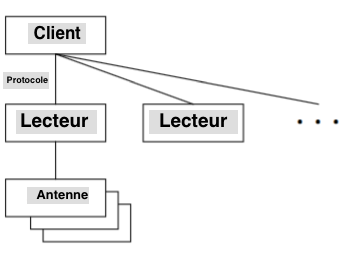
\includegraphics[width=6cm,height=6cm]{lim}
\caption{Illustration du système RFID}
\end{figure}
Comme on le voit sur la figure 3.7, du point de vue de notre protocole, un lecteur contient une collection d'une ou
plusieurs antennes. De plus, les lecteurs employé dans le présent cahier des charges ne sont pas nécessairement en
correspondance un à un avec les dispositifs matériels.
\subsection{Chronologie de fonctionnement du protocole}
Le fonctionnement du protocole ou d'une connexion comporte deux phases: la phase de négociation et la phase exécution.
\subsubsection{Phase de négociation}
Un client et un lecteur devront négocier une version de protocole pris en charge mutuellement pour chaque connexion. Lorsqu'une connexion  est d'abord établi, à la fois le client et le Reader supposent  la version 1. A l'exception les messages de négociation de version, les messages sont envoyés par le Client  jusqu'à ce que le processus de négociation de version est complète. La négociation de la version est effectuée en utilisant des messages prédéfinit est initiée par le Client. Le client demande la version de protocole pris en charge par le Reader, puis détermine une version appropriée pour la connexion (type de message).
 
Une fois qu'une version a été établie à l'aide de cette procédure, tous les messages suivants sont envoyés en utilisant les message prédéfinit par le lecteur. La chronologie de fonctionnement de la phase de négociation  entre un client et un lecteur est représenté sur la figure 3.
\begin{figure}[H]
\centering
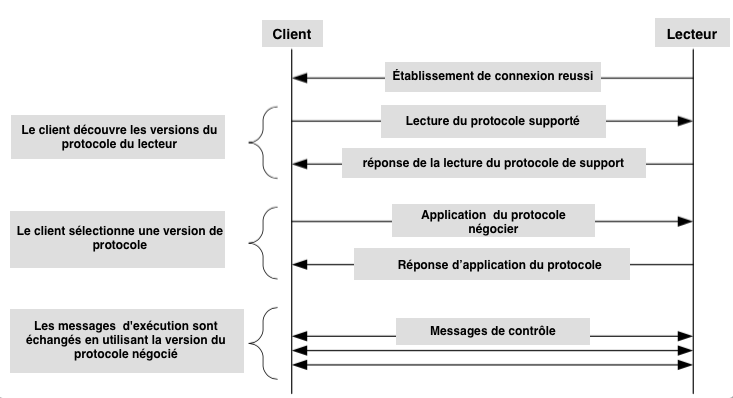
\includegraphics[width=\textwidth]{negotiation2}
\caption{Phase de négociation}
\end{figure}

L'opération d'exécution comprend les phases d'exécution suivantes:
\begin{itemize}
\item découverte des capacités
\item Configuration de l'appareil
\item opérations d'inventaire et d'accès cycles configuration d'inventaire exécutés
\item Si les conditions d'étiquettes adaptées, les opérations d'accès seront exécutés pendant l'exécution du cycle des stocks.
\item  opérations d'accès incluent la lecture, l'écriture et de verrouillage mémoire d'étiquette, étiquettes tuant, etc.
\item Les opérations RF
\item Rapports retournés au Client
\end{itemize}

La figure 3.9 illustre toutes les étape les message échanger entre le lecteur,client et les tags.

Le protocole utilise des unités de données de protocole appelés messages pour communiquer entre le client et le Reader pour  les mises à jour des clients ou pour récupère la configuration du lecteur, en générale pour le contrôle du fonctionnement du lecteur. Cette section nous a donné un aperçu globale du modèle abstrait du protocole, dans le chapitre suivant on va présenter le logiciel qui mis en œuvre ce protocole.
\begin{figure}[H]
\centering
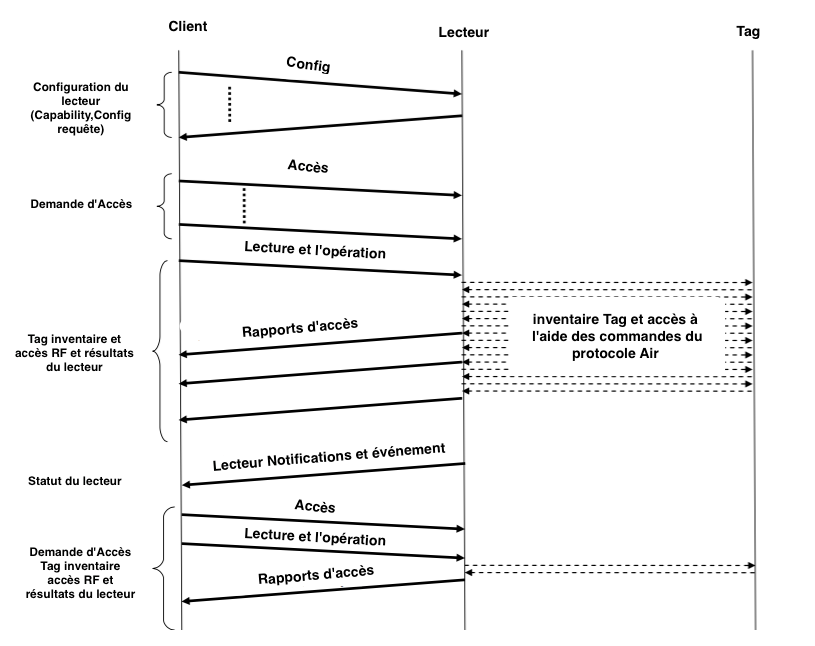
\includegraphics[height=12cm]{runtime}
\caption{Phase d'exécution}
\end{figure}






\section{SmartFlah}
%describe everything you did in The Android
\pagebreak
\section{Antenne UHF}
RFID a des nombreuses applications, une utilisation de cette technologie est pour l'identification des objets dans un stock. Les objets tels que palettes et les cartons sont étiquetés ce façon à lutter contre, le vole et la mauvaise gestion du stock. la détection des objets encapsuler dans les cartons a était une taches impossible sans ouverture des cartons, maintenant avec la RFID cette tâches et devenu une question de quelque seconds.
\subsection{Introduction}
Les étiquettes RFID utilisé au paravent pour cette application sont passifs et surtout opèrent dans le bas fréquence (LF). Cependant, les balises LF ne peuvent être lus qu'a courte portée et peuvent ne pas se comporte bien lorsque plusieurs balises sont simultanément présents dans le domaine.les solution se tourne maintenant vers l'utilisation des tags UHF. tags UHF non seulement donnent une meilleur distance de lecture, mais prennent également en charge des débits plus élevés. \\

Dans cet section, une simple petite étiquette RFID passive opérant dans la fréquence de 915MHz (UHF) est présenté. Dans la section suivante, une brève théorie  sur l'antenne de l'étiquette et la puce utilisée dans notre conception, ainsi que la topologie de la conception théorique et pratique utilisée, suivie d'une discussion sur les points forts de la conception et les détails de sa mise en œuvre pratique avant que des conclusions sont présentées dans la dernière section.
\subsection{Tag antenne et Base du die}
L'antenne choisie pour l'étiquette  est une antenne en boucle. La figure 1 montre une antenne en boucle ayant un diamètre D de la boucle et un fil de diamètre d. Une antenne en boucle est choisie car car elle dispose d'une structre circulaire qui permet de minimiser la taille par rapport au autre technologie comme les middredded et les Microstrip. 

Une antenne dipôle électrique est  non plus possible. le problème du dipôle électrique  demi-onde pour la fréquence de fonctionnement qu'on utilise serait de trop grande taille alors qu'un  petit dipôle électrique peut être utilisé, mais l'expérience montre qu'il est difficile à l'adaptation.
\begin{figure}[H]
\centering
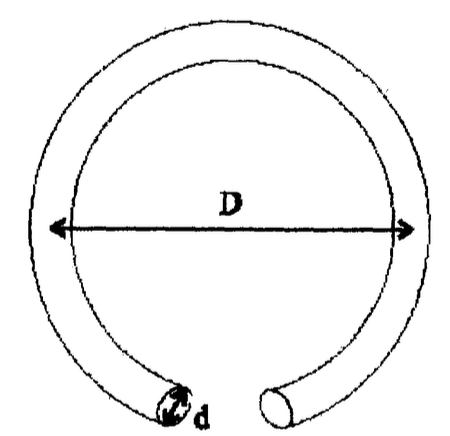
\includegraphics[width=4cm]{cla}
\caption{L'antenne proposée}
\end{figure}

Le circuit équivalent de l'antenne est telle que représentée sur la Figure 3.7 a. En se référant à ce circuit, Rr est la résistance de rayonnement de l'antenne en boucle alors que L est l'inductance de l'antenne à boucle. Dans l'hypothèse de l'uniforme flux de courant, un tour de la résistance de rayonnement R, de l'antenne de la boucle peut être calculée en utilisant l'expression \cite{antennatheory}:

\begin{equation}
R_{r}  = 20 (\pi)^{2}(\beta a)^{4}
\end{equation}
Sur l'hypothèse des courants circulant sur la la surface, l'inductance L de l'antenne peut être calculée en utilisant l'expression suivante \cite{antennatheory}:
\begin{equation}
L  = \frac{\mu_{0}D}{2}[ln(\frac{8D}{d})-2]
\end{equation}

Dans la figue 3.7b montre le circuit équivalent de la puce RFID, qui peut être représenté par une résistance R et d'un condensateur  C en parallèle . R et C utilisé dans l'analyse et la conception de l'étiquette sont 1.3 k\(\Omega\) et 1.15 pF respectivement.

\begin{figure}[H]
\centering
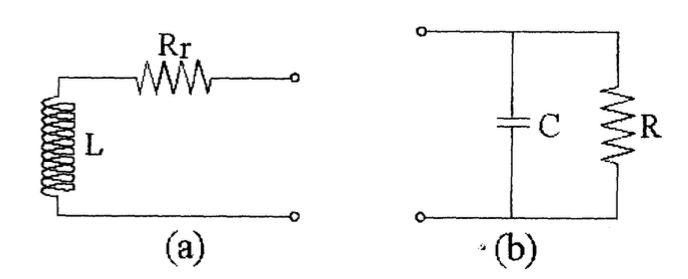
\includegraphics[width=8cm]{eq}
\caption{le circuit équivalent pour (a) une antenne en boucle; (b) RFID tag puce}
\end{figure}

\subsection{Design du Tag}
La fréquence de fonctionnement de l'étiquette se trouve dans la bande UHF.
Aux fins des calculs de conception, la fréquence de 915 MHz a été choisie. Dans la conception initiale, le diamètre de l'antenne de la boucle a été d'environ 2,2 cm à l'aide de 0,2 cm de diamètre fil rond (D = 2.2cmandd = 0.2cm).

En se référant à la figure 3.7a et se référant à l'équation (3.1) et (3.2), la résistance de rayonnement R de l'antenne en boucle peut être calculée pour être de 0,39  \(\Omega\) et la valeur de l'inductance L pour être nH 34,24.\\

Le circuit RC parallèle pour le circuit équivalent de la puce RFID, comme représenté sur la Figure 3.7 b peut être transformer en circuit équivalent en série constitué d'une résistance  R' et une capacité localisée C'. les valeurs R' et C'  peuvent être calculées à environ 17.36 \(\Omega\) et 1,17 pF respectivement sur la base des valeurs R et C indiqué ci-dessus.\\


Par conséquent, à 915 MHz, l'impédance de source, l'impédance à savoir l'antenne, \(Z_{antenne} \) est est de 0,39 ± j199 \(\Omega\) tandis que l'impédance de charge, \(Z_{charge} \) est 17.36-jl49.2 \(\Omega\). On sait que le transfert de puissance maximale se produire lorsque l'impédance de source est égale au conjugué de l'impédance de charge. Par conséquent, un réseau d'adaptation est nécessaire pour obtenir un transfert de puissance raisonnable.\\

Il existe trois réseaux d'adaptation de base utilisés dans les conceptions RF - ils sont L, \(\Pi\) et la configuration T. Chacun d'eux a ses avantages et ses inconvénients. Le réseau d'adaptation plus couramment utilisés est le circuit de L. Les raisons sont les suivantes:
\begin{itemize}
\item Simplicité - Facile à construire des réseaux d'adaptation automatique. Il n'a que deux éléments à contrôler pour ajuster la partie réelle et imaginaire de l'impédance.
\item valeurs de composantes pratiques - certaines des configurations nécessitent soit des valeurs d'inductance très basses ou très hautes valeurs de capacité qui est impossible à faire surtout quand vous devez concevoir réseau d'adaptation automatique avec une gamme très large.\\
\end{itemize}

Le facteur de qualité Q du circuit est déterminée uniquement à partir de la source (générateur) et la charge (impédance du Circuit d'impédance) et ne dépend pas de composants externes - ce qui est peut-être la propriété la plus importante du circuit. Ce que cela signifie est que pour certaine impédance de charge il n'y a qu'une combinaison de L et C pour correspondre à cette charge.
\begin{equation}
Q = \sqrt{\dfrac{R_{source}}{R_{charge}}-1}
\end{equation}

Maintenant, en utilisant la définition de Q à vide pour trouver les séries et parallèles branches.
\begin{equation}
X_{1}=QR_{source}
\end{equation}
\begin{equation}
X_{2}=\dfrac{R_{p}}{Q}
\end{equation}

T et le réseau \(\Pi\) nécessitent une algorithme de contrôle plus complexe pour la conception automatique de réseau d'adaptation. Elle Nécessité de contrôler de trois composants qui le rend plus cher. Et l'inconvénient du circuit de L est qu'elle peut correspondre à des charges égale ou inférieure à 50 Ohm. Si le circuit de L est inversé, il peut correspondre à des charges égale ou supérieure à 50 Ohm. Il ne peut pas correspondre aux des deux côtés. Par exemple, si la charge est en train de changer de 35 à 100 ohms, le réseau de L inversé correspond uniquement à partir de 50 à 100 ohms et ne correspondra pas à 35-50 ohms.
\begin{figure}[H]
\centering
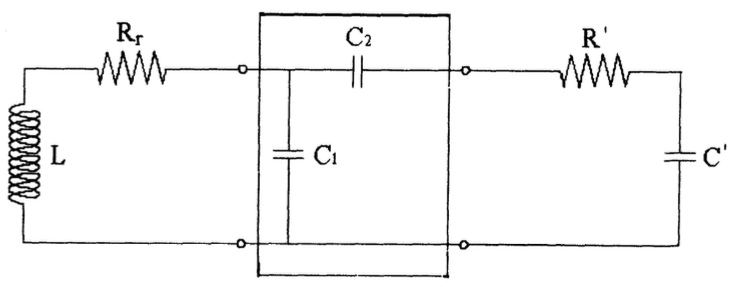
\includegraphics[width=8cm]{matcha}
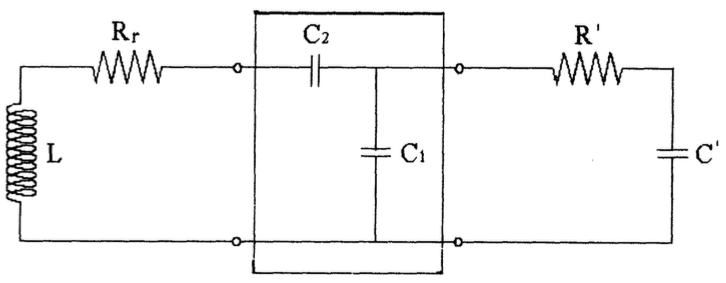
\includegraphics[width=8cm]{matchb}
\caption{Circuit d'adaptation L-shape}
\end{figure}
La figures 3.8 montre deux différents réseaux d'adaptation qui sont utilisés dans notre  design.C1 et C2 peuvent être calculées numériquement ou en utilisant \emph {Smith Chart}. Les valeurs calculées de C1 et C2 pour ces deux topologies que nous considérions sont présentés dans tableau 3.4.\\
\begin{longtable}[c]{| c | c | c |}
 \hline
  & Figure 3.8a & Figure 3.8b\\
 \hline
 \(C_{1}\) / pF & 0.743 pF & 6.557 pF\\
 \hline
 \(C_{2}\) / pF & 0.148 pF & 0.998 pF\\
 \hline
\caption{Réseau d'adaptation}
\end{longtable}
\subsection{Conception de mise en œuvre pratique}
La conception a été démarré à l'aide d'une antenne en boucle et un réseau d'adaptation conçu comme indiqué dans les sections précédentes. L'étape suivante a consisté à examiner la mise en œuvre pratique de l'étiquette. Il a été décidé de mettre en œuvre la conception sur une très mince substrat avec une couche de cuivre sur l'avant côtés. La vue d'arrière du produit final est montré dans la conception figure 3.9. En utilisant le réseau d'adaptation représenté sur la figure. 3.8 b. Cela ne signifie pas que le réseau de d'adaptation représenté sur la figure 3.8a est meilleur que l'autre. Les deux réseaux d'adaptation sont équivalents à la fréquence de résonance, les raisons pour lesquelles l'une représentée sur la figure 3.8b a été choisi était parce qu'il est plus facile à mettre en œuvre par la méthode utilisée ici.

\begin{figure}[H]
\centering
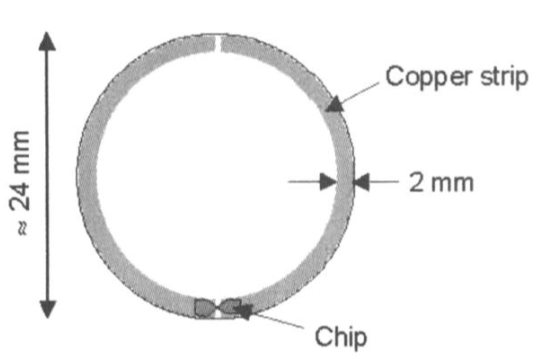
\includegraphics[width=6cm]{front}
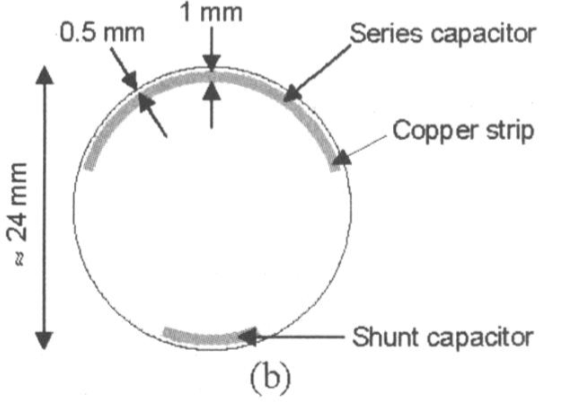
\includegraphics[width=6cm]{back}
\caption{Illustration RFID}
\end{figure}

Cette conception UHF de tag est constitué d'une antenne de boucle circulaire avec un réseau d'adaptation à deux éléments pour faire correspondre les impédances de l'antenne de l'étiquette et l'étiquette puce. Cependant, l'étiquette a été rendue légèrement plus grand diamètre par rapport à celui présenté dans la figure 3.10 en fonction de l'application étudiée. 

Notre conception UHF étiquette (figure 3.10) considérée est constituée d'une antenne à dipôle électrique avec une piste courbe d'inductance à travers le dipôle à des fins d'adaptation d'impédance. La structure et les dimensions de cette balise est représenté sur la figure 3. Cette balise est faite en utilisant une carte FR4 avec une épaisseur de substrat h = 1,6 mm et de permittivité diélectrique \(\epsilon_{r}\) = 4,4. Cette conception de l'étiquette est de simple face.

 La structure d'antenne est simulée en utilisant CST studio 2014 et l'impédance simulée est de 20 + j152 \(\Omega\). Comme on peut le voir, l'impédance de la structure d'antenne de l'étiquette est pas exactement le conjugué de l'impédance de la puce \cite{alien} et donc, l'étiquette et l'impédance de la puce ne sont pas tout à fait adapté.
\begin{figure}[H]
\centering
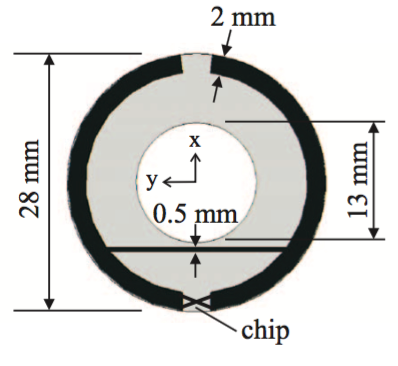
\includegraphics[width=6cm]{dofi}
\caption{UHF étiquette considérée}
\end{figure}

Cependant, la piste d'inductance à travers le dipôle ne fournit pas d'inductance suffisante pour accorder à la capacité de la puce de l'étiquette. Le diagramme de rayonnement de l'antenne, avec un maximum de directivité de 1,83 dB. Comme on le voit sur la section de simulation, bien que la forme générale du motif de rayonnement du première et seconde étiquettes UHF est presque identique, la directivité maximale de ces deux balises se produisent à différentes directions par rapport au plan des étiquettes. Les deux tags UHF ne sont pas testés et les résultats théorique de la distance de lecture sont présentés dans le tableau 3.5.

\begin{longtable}[c]{| c | c | c |}
 \hline
  & UHF tag 1 & UHF tag 2 \\
 \hline
 Tag dans l'espace libre & 1.00 & 0.48\\
 \hline
 Tag attaché à la main  & 0.20 & 0.27\\
 \hline
\caption{Distance de lecture}
\end{longtable}
\subsection{Minaturisation des antenne CLA}
Le cahier de charge impose par la nature de la solution  a concevoir une antenne de petite taille (>2cm), la radiation doit être dans la bande autorise par l'ANRT et la puissance reçu au niveau de la puce doit êtres suffisante pour alimenter le circuit. Les deux antenne précédemment présenter en une taille relativement grand et les résultat de la simulation prédicte une mauvaise alimentation du circuit de la puce. donc on a était obliger de penser a une solution pour réduire la taille et améliorer les performance de l'antenne. La littérature \cite{stub}  propose une solution possible qui peut
miniaturiser une antenne en boucle circulaire (CLA) à l'aide de \emph{short stubs} insérés dans la partie interne de la boucle. Dans le cas d'une longueur d'onde et une demi-longueur d'onde, respectivement, l'antenne est réduite jusqu'à 83\% et 92,1\% de sa taille par rapport au type CLA général. Par ailleurs la perte de retour, la bande passante -10dB et le gain d'une longueur d'onde et une demi-longueur d'onde sont de 12MHz (1,3\%), et de 48MHz (5\%). la deuxième méthode sera présenter dans avec la partie simulation dans le chapitre suivant.\\

La figure 3.11 présente des caractéristiques de changement de fréquence de résonance lorsqu'un \emph{short stubs} est mis en œuvre à l'intérieur de la boucle de l'antenne. La longueur du  \emph{short stubs} est de 20 mm et la fréquence de résonance chute 30MHz (3,3\%) à partir de 911.25MHz à 881.25MHz lorsque l'écart de la ligne est 2mm. En effet, le courant est distribué le long la longueur totale de la boucle est augmentée à 13\%. En outre, non seulement les capacitances sont augmentées par la dilatation de la longueur de la boucle, mais aussi les inductances sont augmentées par la structure de \emph{short stubs}. Par conséquent, l'impédance de l'antenne permet une adaptation d'impédance que la longueur de boucle est supérieure à une longueur d'onde,de sorte que la fréquence est éventuellement diminuée. Si elle est résonant à la même fréquence, le diamètre total de la boucle devient plus petit, de sorte que l'antenne cadre est miniaturisé par les bouts joints.


\begin{figure}[H]
\centering
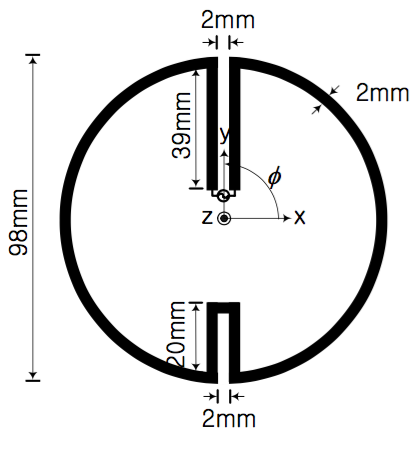
\includegraphics[width=6cm, height=6cm]{stuba}
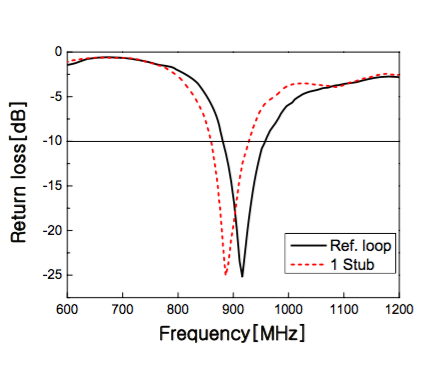
\includegraphics[width=6cm, height=6cm]{stubb}
\caption{CLA - S11}
\end{figure}

\begin{figure}[H]
\centering
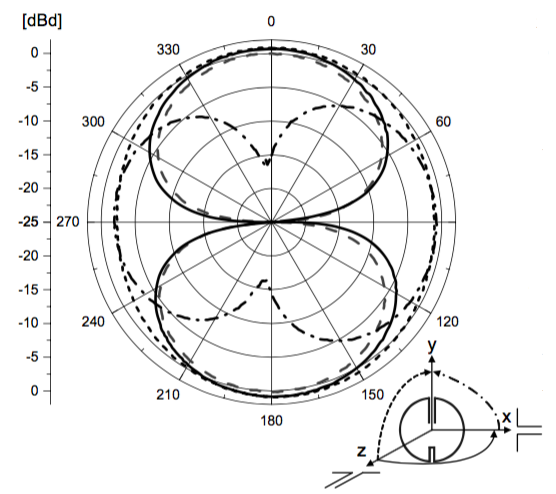
\includegraphics[width=6cm]{lob}
\caption{far-field pattern avant miniaturisation}
\end{figure}

Au moyen du procédé de miniaturisation de l'antenne en boucle, l'antenne de la figure 3.11 est miniaturisé avec des \emph{short stubs} de 11,5 mm et 7 mm . La largeur de la ligne est de 0.3mm et l'intervalle entre les lignes est de 0.3mm. Il est adapté à la longueur et l'intervalle de la ligne d'alimentation est de 8mm et 1mm. Le diamètre d'une antenne est miniaturisé à 40 mm.\\
\begin{figure}[H]
\centering
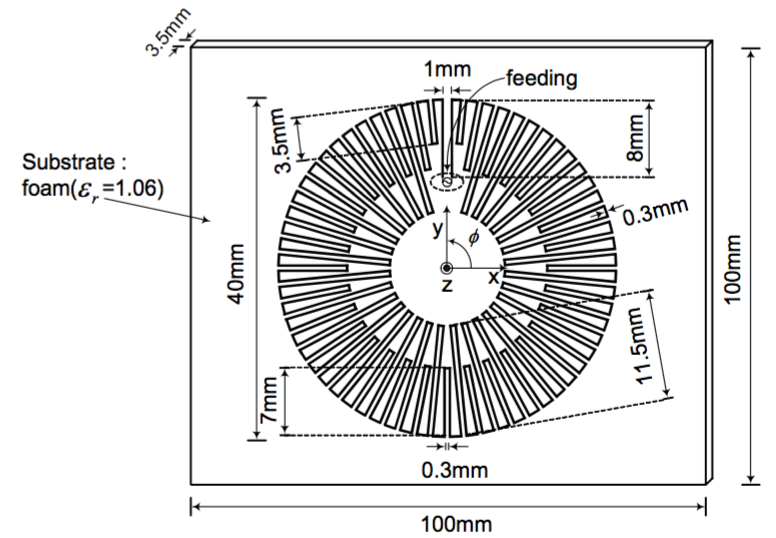
\includegraphics[width=6cm]{structure}
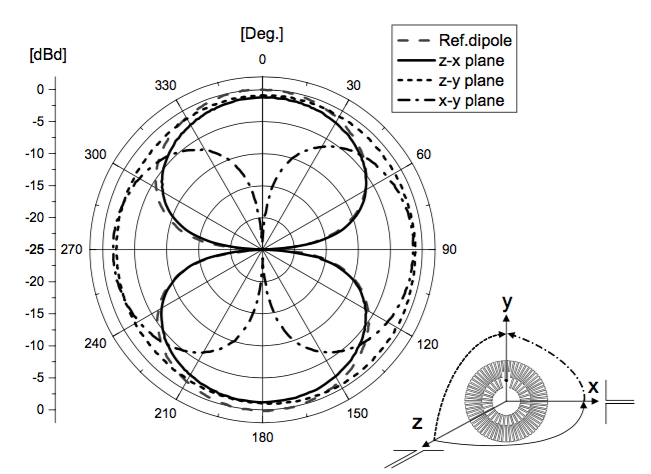
\includegraphics[width=6cm]{structurea}
\caption{CLA après miniaturisation}
\end{figure}

Une autre méthode a était conçu après des expérience de \emph{Reverse Engineering} des tag UHF acheté du marche. cette méthode consiste a boucle l'antenne en interne de tell sorte a minimiser le diamètre sans changer la longueur les deux pôles. la figure suivante présente les résultats de l'analyse par  \emph{X-RAY Reverse engineering} qui permet de voire en interne sans massacre la pièce. Le figure suivante présente les résultats du \emph{Reverse engineering}. L'étiquète est constituer de deux couche de cuivre, la puce est fixé sur l'antenne fixage avec \emph{wire bonding}. la simulation de cette antenne sera présenter dans le chapitre suivant. \\

\begin{figure}[H]
\centering
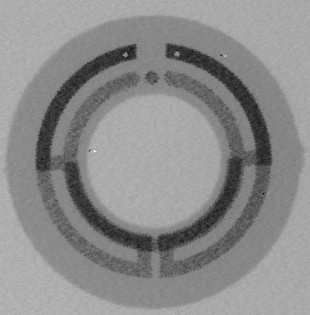
\includegraphics[width=6cm]{xray}
\caption{X-Ray du tag UHF}
\end{figure}

On c'est inspirer de cette méthode qu'on appellerait dans ce rapport \emph{bouclage interne} pour améliorer notre antenne et l'optimiser au niveaux de taille. le figure suivante montre la nouvelle version de l'antenne en figure 3.15. la taille a était réduite de 30 \% on a passé de 28 mm a 22 mm. la nouvelle structure permet un contrôle facile de fréquence et d'impédance. dans les section qui suite on présente une étude détaille sur les avantage de cette nouvelle structure et aussi quelque amélioration qui nous a permise de descendre encore plus base en terme de diamètre de l'antenne. Une étude plus parfondis a était consacre sur cette base a fin de relever toutes les secrètes de cette méthode.\\

\begin{figure}[H]
\centering
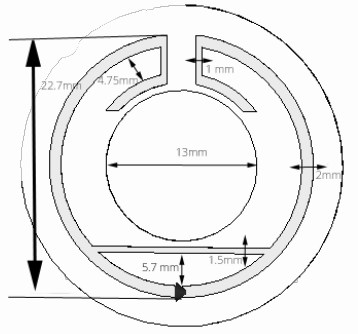
\includegraphics[width=6cm]{1STee}
\caption{Tag UHF améliorer}
\end{figure}
Comme le montre la figure 3.15 la taille a était énormément améliorer et les performance de cette antenne gardant les même. cette structure nous a permit un bon contrôle de fréquence. toute variation de longueur de 2mm nous donne un décalage de fréquence de 10MHz. La figure 3.16 est le S11 après chaque coupage de boucle intérieur de 2mm.plus de détail sur la simulation seront présenter dans le chapitre suivant.\\

\begin{figure}[H]
\centering
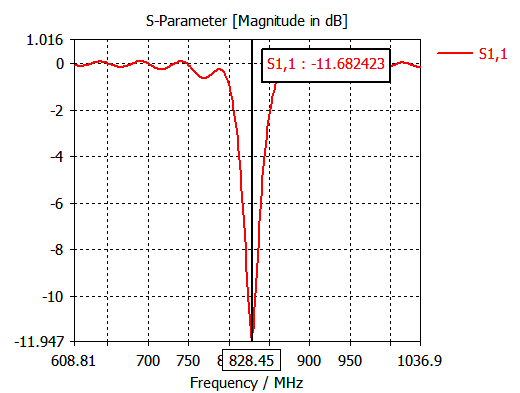
\includegraphics[width=6cm]{11}
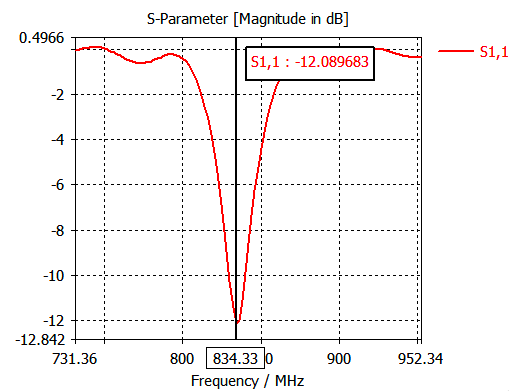
\includegraphics[width=6cm]{22}\\
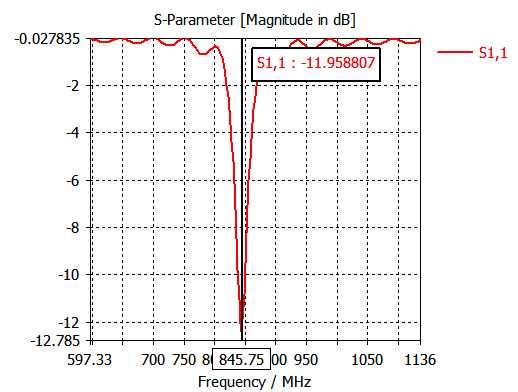
\includegraphics[width=6cm]{33}
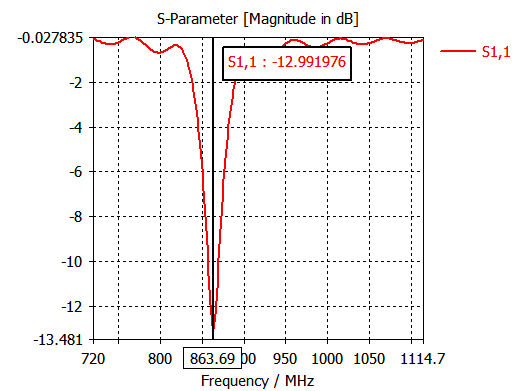
\includegraphics[width=6cm]{44}
\caption{S11 apres coupage de 2mm }
\end{figure}

La troisième étape  consiste a réaliser l'antenne de la figure 3.17. 
Avant de concevoir un prototype de tag RFID destiné à la traçabilité des palettes, un modèle a été mis à notre disponibilité pour être analysé dans les laboratoires de MAScIR.Le but de cette analyse est de caractériser le produit et de déterminer les différents matériaux utilisés.\\

Pour faire on comance pare une Analyse non destructive qui consiste a faire une analyse générale  du boitier puis une description générale du package vu de l’extérieur,Puis avec les Rayons X comme illustre la figure 3.14. En suite on procede a une l'analyse destructive qui consiste a décapsulation le package puis faire une décapsulation du System.



Dans la figure suivante.Cette structure a était inspire de l'analyse avec x-ray d'une antenne acheté du marche qui rayonne dans la fréquence 915MHz. l'expérience montre que sa distance de lecture est de 2m.plus de détail sur la simulation seront présenter dans le chapitre suivant.\\

\begin{figure}[H]
\centering
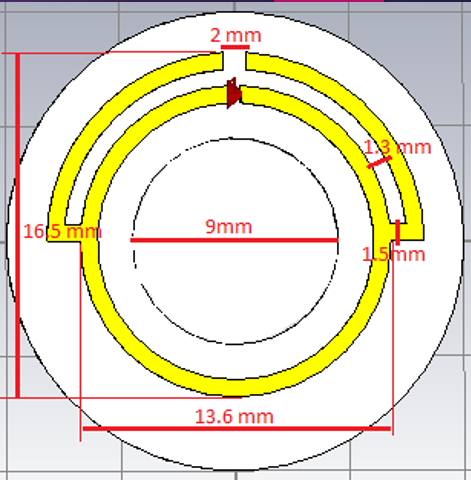
\includegraphics[width=4cm]{front11}
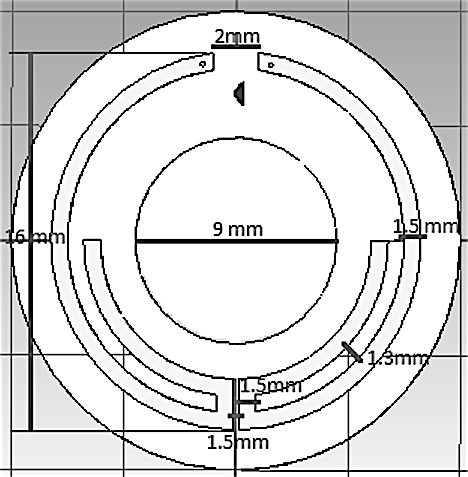
\includegraphics[width=4cm]{back22}
\caption{S11du tag UHF améliorer }
\end{figure}

Dans cette section on a discuter les notion théorique qui régie les antenne a boucle circulaire qui représente une excellente solution pour les antenne de petite taille. Une étude sur les méthode d'optimisation on était détaille dans cette section comme le \emph{Short stub} et le bouclage interne qui permettent de réduire la taille et garder le caractère omnidirectionnel, après cette étape on a élaboré un plan d'expérience qui consiste a examiner une tag achète du marche et puis l'analyser avec un \emph{X-RAY} pour s'inspirer de sa structure. le produit final de cette étude est une tag UHF marocaine d'excellente performance.
\section{conslution}


\chapter{Réalisaion et simulation du projet}
Dans ce chapitre je présente les outils	de	réalisation	et de	simulation en suite la réalisation	du projet et les étape de test	 et vérification et finalement un plan de mise en œuvre et plan de maintenance.
\section{Outils	de	réalisation	et de	simulation}
\subsection{Visuel Studio et .net C sharp}
\subsubsection{Visuel Studio}
\subsubsection{.net C sharp}
\subsection{Android Studio}
\subsection{CST studio}

\section{Réalisation	du	projet}
\subsection{Antenne UHF}

Pour décrire la performance d'une antenne , les définitions des différents paramètres sont nécessaires . Certains paramètres sont interdépendants et pas tous d'entre eux doivent être indiquées pour une description complète de la performance de l'antenne. La définitions des paramètres seront donnés dans section suivante. Beaucoup de ceux sont des standard IEEE  ( IEEE Std 145-1983 ). Ensuite je vais présenter les différentes résultats et simulation sur les antennes RFID UHF. La puce utiliser est la H3 de Alien. Le logiciel de simulation est CST studio 2014 qui permet de calculer un grand nombre des paramètres d'antenne.\\
\subsubsection{Les paramètres de l'antenne}
\begin{itemize}
\item \emph{RADIATION PATTERN}
Un motif de motif ou une antenne rayonnement de l'antenne est définie comme : une fonction mathématique ou d'une représentation graphique des propriétés de rayonnement de l' antenne en fonction des coordonnées spatiales. Dans la plupart des cas, le diagramme de rayonnement est déterminée dans la région de champ \emph{Far-Field} est représentée comme une fonction des coordonnées de direction . Propriétés de rayonnement comprennent la densité de flux de puissance , l'intensité du rayonnement, l'intensité du champ , directivité , de phase ou de polarisation.
\begin{figure}[H]
\centering
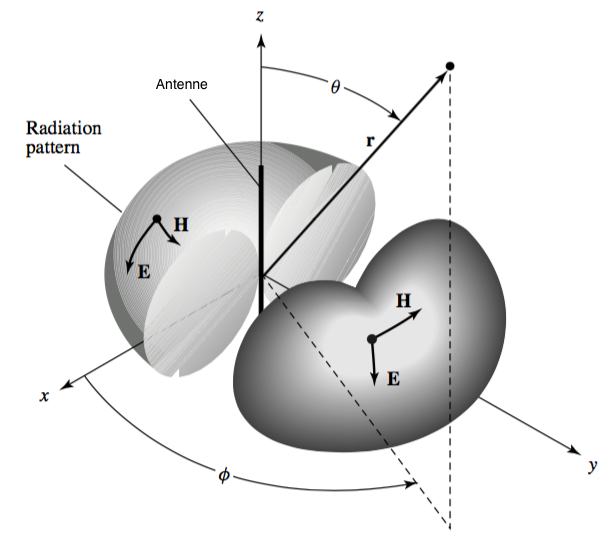
\includegraphics[width=5cm,height=5cm]{radpa}
\caption{Radiation pattern}
\end{figure}
\item \emph{la directivité} la directivité d'une antenne est définie comme: le rapport de l'intensité du rayonnement dans une direction donnée de l'antenne à l'intensité de rayonnement moyenne de toutes les directions. L'intensité de rayonnement moyenne est égale à la puissance totale rayonnée par l'antenne divisée par 4\(\pi\) .En forme mathématique elle peut être écrit comme:

\begin{equation}
D = \dfrac{U}{U_{0}} = \dfrac{4 \pi U}{P_{rad}}
\end{equation}

Si la direction n'est pas spécifiée, elle implique la direction de l'intensité maximale de rayonnement( Directivité maximum) exprimé comme:

\begin{equation}
D_{max} = D_{0} = \dfrac{U}{U_{0}} = \dfrac{4 \pi U_{max}}{P_{rad}}
\end{equation}
D = directivité (sans dimension)\\
\(D_{0}\) = directivité maximale (sans dimension)\\
U = intensité du rayonnement ( W / unité d'angle solide )\\
\(U_{max}\) = intensité maximale de rayonnement ( W / unité d'angle solide )\\
\(U_{0}\) = intensité du rayonnement de la source isotrope ( W / unité d'angle solide ) Prad = puissance totale rayonnée ( W )\\

\item \emph{EFFICACITÉ}

elle peut êtres définit comme suite: \emph{comment bien l' antenne rayonne la puissance qui lui est donné.} Le total efficacité de l'antenne est utilisée pour prendre en compte les pertes au niveau des bornes d'entrée et à l'intérieur de la structure de l'antenne. Ces pertes peuvent être dues  à la réfection en raison de mal adaptation entre la ligne de transmission et la source de l'antenne, la conduction et diélectrique

\begin{figure}[H]
\centering
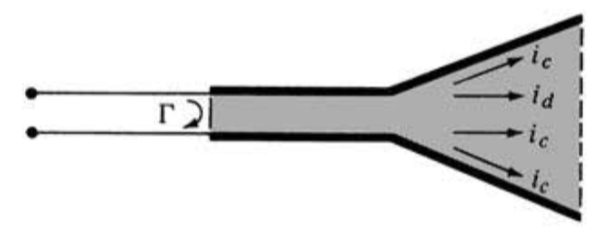
\includegraphics[width=4cm,height=3cm]{wellwellwell}
\caption{réflexion,conduction,perte de diélectrique}
\end{figure}
D'une manière générale , le rendement global peut être écrite comme:

\begin{equation}
e_{0}=e_{r}e_{c}e_{d}
\end{equation}

\(e_{0}\) = l'efficacité totale ( dimension)\\
\(e_{r}\) = réflexion \emph{ mismatch} \\
\(e_{c}\) = l'efficacité de conduction ( sans dimension)\\
\(e_{d}\) = efficacité diélectrique ( sans dimension)\\

\item \emph{VSWR} 
Pour une radio ( émetteur ou récepteur ) pour délivrer une puissance à une antenne , l'impédance de la ligne de transmission radio et doit être bien adaptée à l'impédance de l'antenne . Le paramètre ROS ou VSWR est une mesure qui décrit numériquement la façon dont l' antenne a une adaptation d'impédance à la ligne de la radio ou de la transmission , il est connecté.
\begin{equation}
VSWR = \dfrac{1+ |\Gamma|}{1-|\Gamma|}
\end{equation}

\item \emph{S paramètres}
décrivent la relation d' entrée-sortie entre les ports (ou terminaux) dans un système électrique . Par exemple, si nous avons 2 ports ( intelligemment appelé Port 1 et Port 2), puis S12 représente la puissance transférée de Port 2 à Port 1. S21 représente la puissance transférée de Port 1 à Port 2. En général, SNM représente la puissance transférés de Port M à Port N dans un réseau multi- port.
\end{itemize}

\subsubsection{Le premier prototype UHF}


La conception UHF étiquette considérée est constituée d’une antenne à dipôle électrique avec une piste courbe d’inductance à travers le dipôle à des fins d'adaptation d'impédance. La structure et les dimensions de cette balise est représenté sur la figure 3. Cette balise est faite en utilisant une carte FR4 avec une épaisseur de substrat h = 1,6 mm et de permittivité diélectrique \(\epsilon_{r}\) = 4,4. Cette conception de l’étiquette est de simple face.

 l'impédance simulée est de 20 + j152 \(\Omega\).l'impédance de la structure d'antenne de l'étiquette est pas exactement le conjugué de l'impédance de la puce [6] et donc, l'étiquette et l'impédance de la puce ne sont pas tout à fait adapté.\\
 
 \begin{figure}[H]
\centering
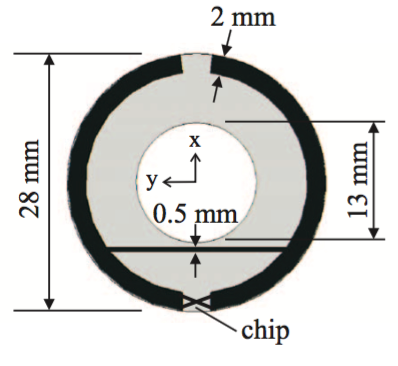
\includegraphics[width=6cm]{dofi}\\
\caption{Paramettre de sumulation CLA}
\end{figure} 

Les figures suivante représente les quatre importante paramétrés a prendre en considération pour le jugement d'une antenne. la première valeur est la s11
\begin{figure}[h]
\centering
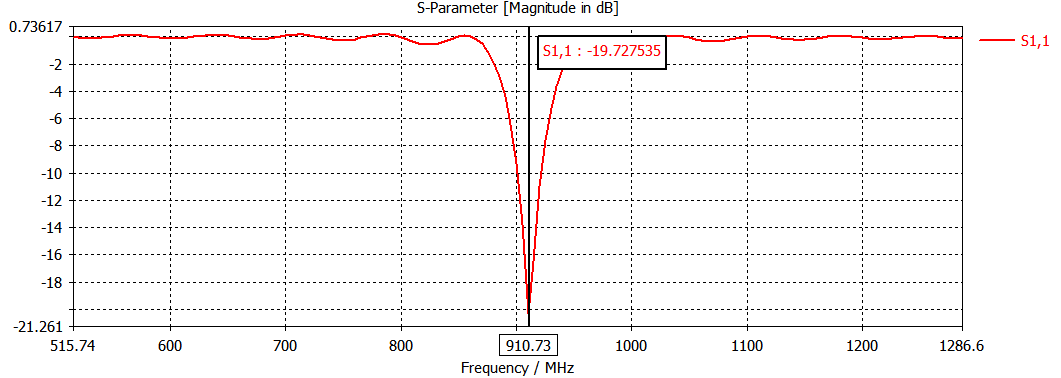
\includegraphics[width=6cm,height=3cm]{clas11}
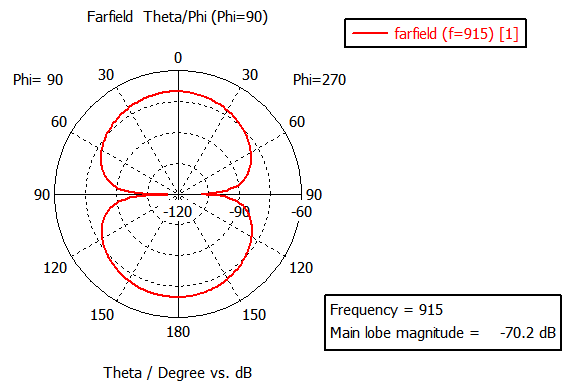
\includegraphics[width=6cm,height=3cm]{clapolfarfield}
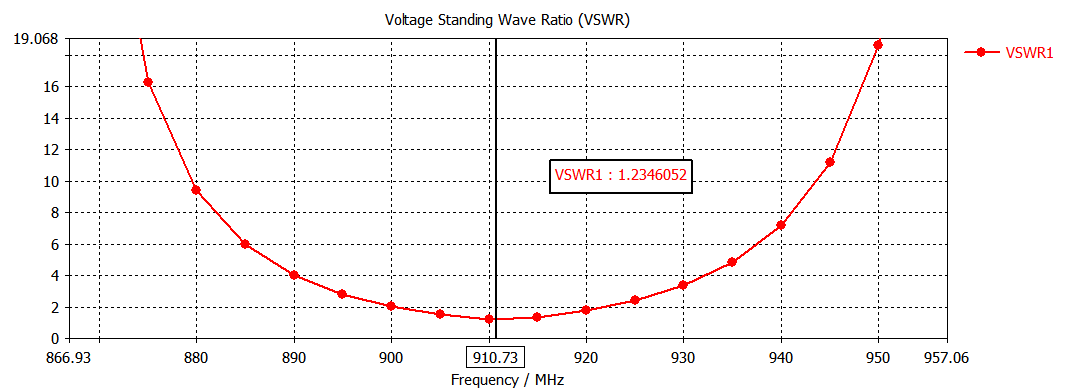
\includegraphics[width=6cm,height=3cm]{clavswr}
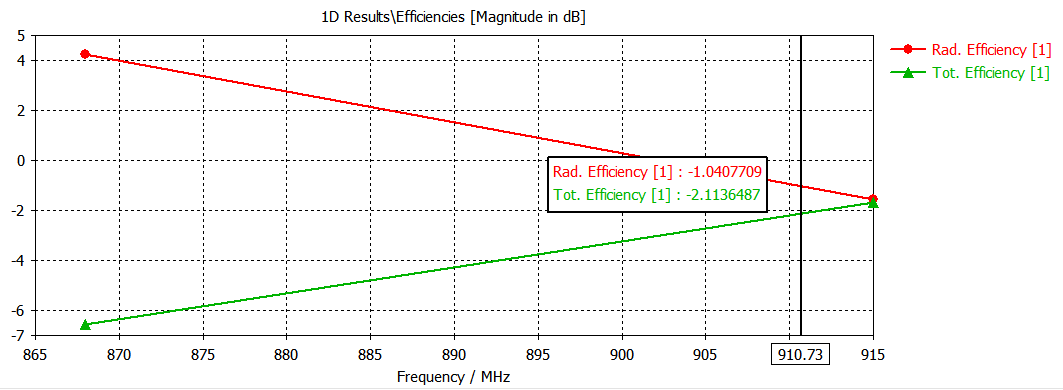
\includegraphics[width=6cm,height=3cm]{claefficency}
\caption{Paramettre de sumulation CLA}
\end{figure} 
%talke about seuille values and compared them to what we got
% bandwith power related to s11, (feathers or capabilities)

\subsubsection{L'antenne a boucle circulaire}
La structure suivante représente  la forme améliorer de l'antenne précedante, cette structure nous a permit de réduire la taille et donner la main sur un contrôle totale de fréquence. l'impédance de l'antenne simuler est  de 27 + j18\(\Omega\)
.
\begin{figure}[H]
\centering
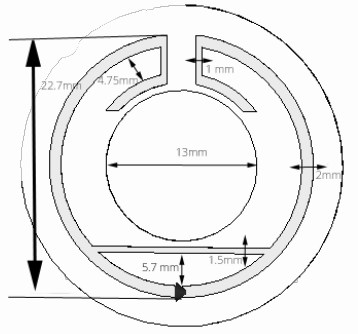
\includegraphics[width=6cm]{1STee}
\caption{antenne a boucle circulaire}
\end{figure}
Les figures suivante représente les quatre importante paramétrés a prendre en considération pour le jugement d'une antenne.

\begin{figure}[h]
\centering
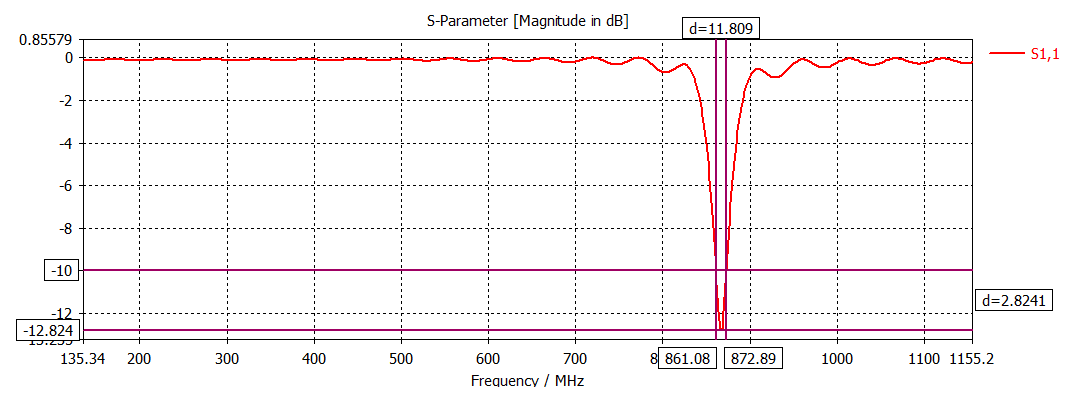
\includegraphics[width=6cm,height=3cm]{claaaass11}
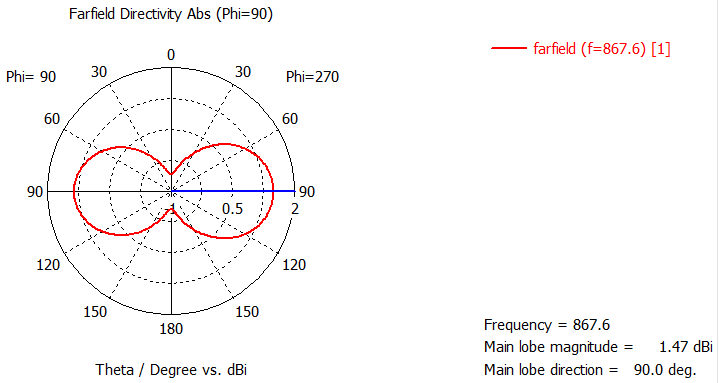
\includegraphics[width=6cm,height=3cm]{claPattern}
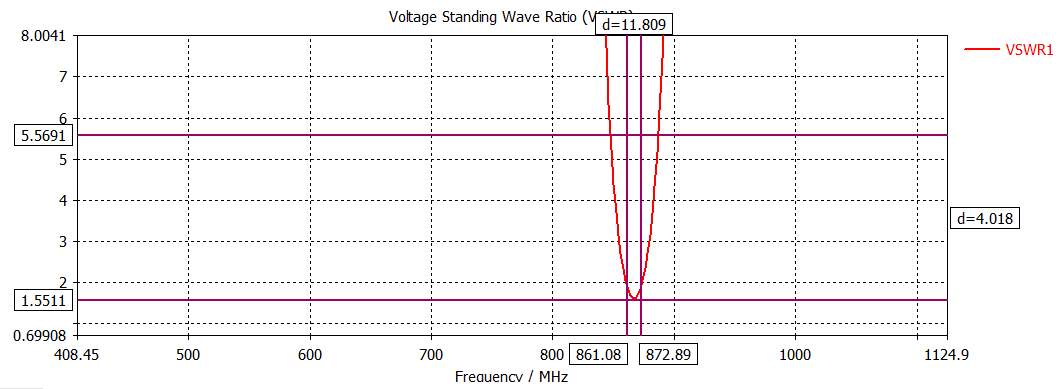
\includegraphics[width=6cm,height=3cm]{claaavswr}
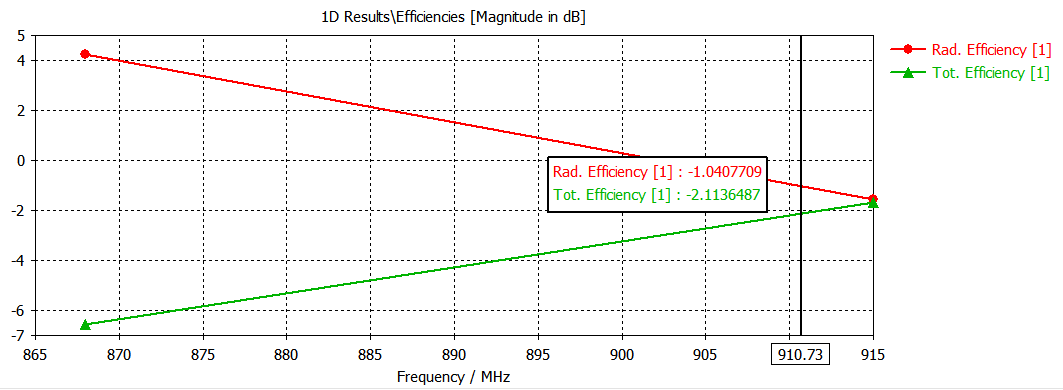
\includegraphics[width=6cm,height=3cm]{claefficency}
\caption{Paramettre de sumulation CLA}
\end{figure} 
%talke about seuille values and compared them to what we got
% bandwith power related to s11, (feathers or capabilities)


\subsubsection{L'antenne a boucle circulaire}
la figure suivante présente les résultats de l'analyse par  \emph{X-RAY Reverse engineering} qui permet de voire en interne sans massacre la pièce. Le figure suivante présente les résultats du \emph{Reverse engineering}. L'étiquète est constituer de deux couche de cuivre, la puce est fixé sur l'antenne fixage avec \emph{wire bonding}. la simulation de cette antenne sera présenter dans le chapitre suivant. \\

\begin{figure}[H]
\centering
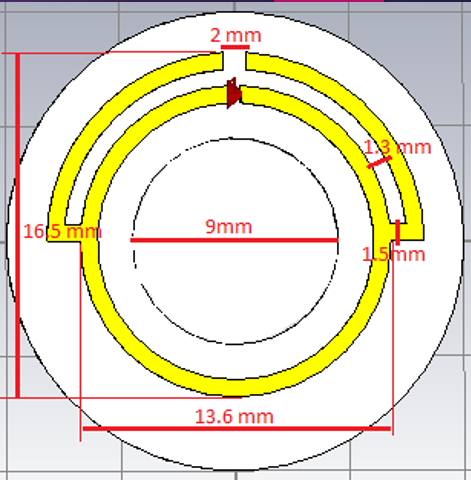
\includegraphics[width=4cm]{front11}
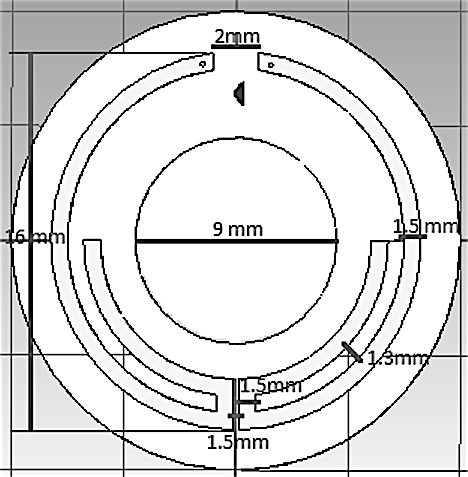
\includegraphics[width=4cm]{back22}
\caption{S11du tag UHF améliorer }
\end{figure}

Les figures suivante représente les quatre importante paramétrés a prendre en considération pour le jugement d'une antenne.

\begin{figure}[h]
\centering
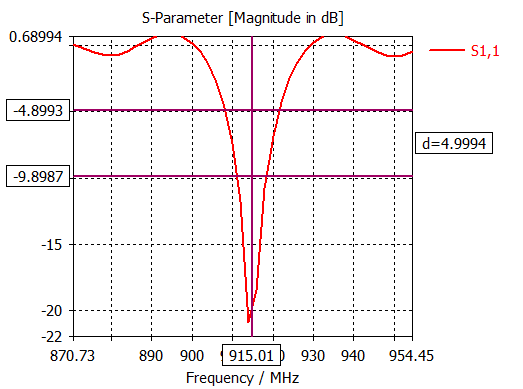
\includegraphics[width=6cm,height=3cm]{uses11}
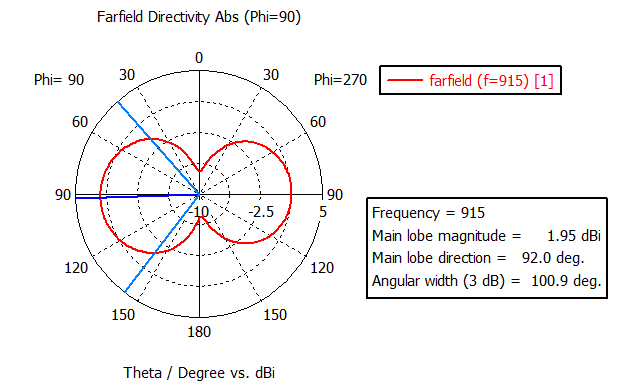
\includegraphics[width=6cm,height=3cm]{usefar}
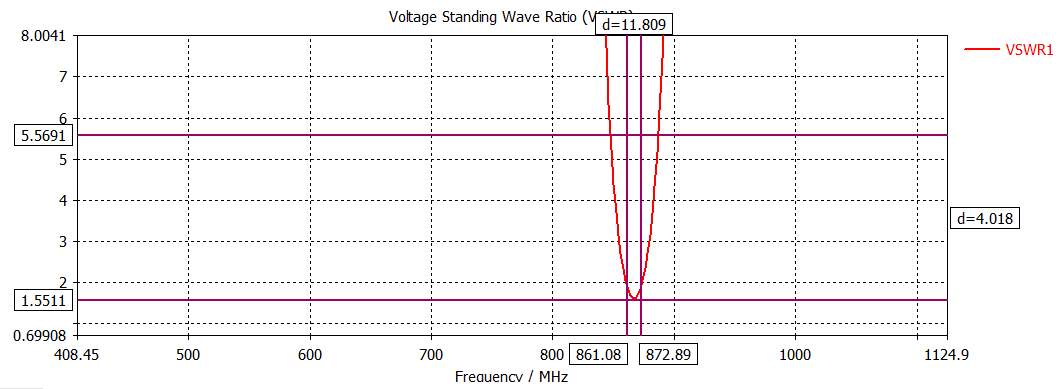
\includegraphics[width=6cm,height=3cm]{claaavswr}
\includegraphics[width=6cm,height=3cm]{useeff}
\caption{Paramettre de sumulation CLA}
\end{figure} 
%talke about seuille values and compared them to what we got
% bandwith power related to s11, (feathers or capabilities)

\subsubsection{antenne a boucle circulaire (CLA)}

\section{Test	 et vérification	}
\section{Mise en	œuvre	 et	plan	de	de maintenance	}
		
\begin{thebibliography}{9}

\bibitem{antennatheory} 
C. A. Balanis, "Antenna Theory: Analysis and
Design",2ndEdition,1997,JohnWiley and Sons.
 



\bibitem{j}  J. Landt, “The history of RFID,” Potentials, IEEE, vol. 24, no. 4, pp. 8–11, 2005.

\bibitem{stub} Small Circular Loop Antenna for RFID Tag
Hong-Kyun Ryu and Jong-Myung Woo
Department of Radio Science and Engineering, College of Engineering, Chungnam National University, Daejeon, Korea

\bibitem{G} G. S. Pope, M. Y. Loukine, D. M. Hall, and P. H. Cole, “Innovative systems de- sign for 13.56 MHz RFID,” in Wireless and Portable Design Conference, Burling- ton, Massachusetts, 1997, pp. 240–245.

\bibitem{texas}  Texas Instruments, “Tag-it HF-I standard transponder IC - reference guide,” 15 Jan. 2007. 

\bibitem{alien}  “HF antenna design notes,” Technical Application Report, 2003.
[7] Alien Technologies, “915MHz EPC Class 1 RFID tags,” 15 Jan. 2007. [Online]. Available: http://www.alientechnology.com/products/documents/
alien 915mhz 128 bit.%pdf

\bibitem{fromat}  EPCglobal Tag Data Standards Version 1.3 Ratified Specification
March 8, 2006

\bibitem{air} EPC™ Radio-Frequency Identity Protocols Generation-2 UHF RFID
Specification for RFID Air Interface Protocol for Communications at 860 MHz – 960 MHz 
Version 2.0.0 Ratified

\end{thebibliography}



\end{document}